\chapter{Modelo Matemático} \label{ch:mathematical_model}

Segundo \citeonline{bib:maliska}, a solução numérica de qualquer problema físico requer a sua prévia modelagem matemática. Um modelo matemático é uma representação de um sistema real através de equações. Essas equações são obtidas ao se fazerem hipóteses sobre o comportamento do sistema estudado, e a representatividade do modelo depende das simplificações feitas nesse processo.

Este capítulo aborda os aspectos matemáticos pertinentes ao Método de Elementos Discretos. São abordados os principais conceitos referentes aos sistemas de partículas, e apresentadas as equações de movimento que governam o problema. Os principais modelos de força de colisão são então expostos e, por fim, é apresentado o algoritmo de Gear, responsável por resolver as equações.

\section{Sistemas de Partículas} \label{sec:particle_systems}

As partículas são os elementos fundamentais do Método de Elementos Discretos. De acordo com a definição apresentada por \citeonline{bib:sampaio}, partículas são consideradas corpos rígidos. Por serem indeformáveis, fica implícita a hipótese de que não ocorrem deformações plásticas nesses elementos, e então eles preservam a sua geometria mesmo durante e após colisões.

A princípio, o \DEM{} suporta geometrias arbitrárias para seus elementos. Entretanto, devido a limitações de modelos físicos e de avaliação das colisões, em geral consideram-se formatos básicos como esferas, superelipsoides e poliedros. Geometrias mais complexas podem ser geradas pela associação de geometrias mais simples em partículas compostas \cite{bib:sampaio,bib:computational_granular_dynamics}.

Um sistema de partículas é, por sua vez, um conjunto de partículas que interagem entre si. Considera-se que o sistema possua um referencial global fixo centrado no ponto \(\originPoint\) a partir do qual as demais grandezas vetoriais são definidas.

A cada partícula está associada uma função posição que determina, vetorialmente, a posição de seu centro de massa com relação à origem do sistema. A orientação de um elemento é a orientação do seu sistema de eixos principais com relação ao sistema global. Com isso, cada partícula possui seis graus de liberdade: três translações e três rotações \cite{bib:sampaio}. Os elementos discretos ainda contêm diversas \textit{propriedades}, as quais são determinantes para as suas interações.

As translações e rotações das partículas são determinadas através da solução das equações de movimento, detalhadas na seção \ref{sec:equations_of_motion}. Essas equações dependem das interações que ocorrem entre as partículas. Em um sistema qualquer, as interações podem ser de diversas naturezas, tais quais colisões mecânicas, troca de cargas elétricas, transferência de calor, e outras. No entanto o \DEM{} considera, a princípio, apenas as colisões e as forças de campo, como a gravidade.

Embora a quantidade de elementos em um sistema seja arbitrária, ela é sempre finita. Denotando por \(\numberOfParticles\) essa quantidade, é possível enumerarem-se esses elementos e definir-se o conjunto de partículas do sistema como
\begin{equation*}
	\particleSet = \left\lbrace\particlei \suchThat 1\leq i\leq\numberOfParticles\right\rbrace,
\end{equation*}
sendo \(\particlei\) a \(i\)-ésima partícula no sistema.

Cada partícula ainda possui uma \textit{vizinhança}, que é o conjunto de elementos que podem interagir com ela. Denota-se por \(\ineighborhood{i}\) ou \(\neighborhoodOf{\particlei}\) a vizinhança da partícula \(i\). A determinação da vizinhança de uma partícula é essencial para o cálculo das forças e dos torques que atuam sobre ela, e alguns dos métodos para se construir esse conjunto são apresentados na \autoref{sec:neighborhood}.

Escrevendo como \(\forceji\) a força e \(\torqueji\) o torque aplicados pela partícula \(\particlej\) sobre a partícula \(\particlei\), tem-se que a força resultante \(\resultingForcei\) e o torque resultante \(\resultingTorquei\) sobre \(\particlei\) são dados pelo princípio da superposição como
\begin{gather}
	\resultingForcei = \sum_{\particlej\in\ineighborhood{i}}\forceji + \external\resultingForcei, \label{eq:superposition_translation} \\
	\resultingTorquei = \sum_{\particlej\in\ineighborhood{i}}\torqueji + \external\resultingTorquei, \label{eq:superposition_rotation}
\end{gather}
em que \(\external\resultingForcei\) e \(\external\resultingTorquei\) são a força e o torque \textit{externos} atuantes sobre \(\particlei\), isto é, resultantes da interação entre a \(i\)-ésima partícula com elementos exteriores ao sistema.

Uma importante hipótese que se faz no Método de Elementos Discretos é que a interação entre duas partículas \(\particlei\) e \(\particlej\) não interfere na interação entre outras partículas ou entre \(\particlei\) e uma terceira partícula \(\particlek\). Com isso, cada par de partículas pode ser estudado isoladamente, e o estado final do sistema, após as interações, é uma simples combinação desses resultados.

\section{Equações de Movimento} \label{sec:equations_of_motion}

Na dinâmica de partículas, os elementos estudados são considerados corpos rígidos, aos quais se aplicam as leis de Euler para o movimento \cite{bib:sampaio, bib:dynamics_of_multibody_systems}.

Em um sistema inercial fixo, considera-se uma partícula de massa \(\mass\) com um centro de massa \(C\) cuja posição é descrita pela função vetorial \(\position\). Além disso, considera-se que a partícula possua uma velocidade angular \(\angularVelocity\) e um tensor momento de inércia \(\tensorOfInertia\) definido com relação ao seu centro de massa.

Conforme demonstrado por \citeonline{bib:dynamics_of_multibody_systems}, a \textit{quantidade de movimento linear} e a \textit{quantidade de movimento angular} da partícula, denotadas respectivamente por \(\linearMomentum\) e \(\angularMomentum\), são então dadas por
\begin{gather*}
	\linearMomentum = \mass\cdot\velocity, \\
	\angularMomentum = \position\cross\linearMomentum + \tensorOfInertia\cdot\angularVelocity.
\end{gather*}

\subsection{Primeira Lei de Euler}

A primeira lei de Euler trata do movimento de translação. Ela se expressa através da equação
\begin{equation} \label{eq:euler_first}
	\resultingForce = \deriv{1}{\linearMomentum},
\end{equation}
sendo \(\resultingForce\) o vetor força resultante sobre a partícula. Para o caso em que a massa do corpo é constante, a primeira lei de Euler torna-se equivalente à segunda lei de Newton:
\begin{equation} \label{eq:motion_first}
	\resultingForce = \mass\cdot\acceleration.
\end{equation}

A equação \eqref{eq:euler_first} é aplicada para os fenômenos de fragmentação e aglutinação, casos em que partículas são divididas ou unidas, sendo que a massa de cada partícula isoladamente não é constante. \citeonline{bib:computational_granular_dynamics} apresentam métodos que descrevem o fenômeno de fragmentação. Tais situações, porém, são tratadas separadamente, de modo que a equação \eqref{eq:motion_first} é a que se considera para o estudo da evolução do sistema.

De acordo com o princípio da superposição, a força resultante sobre a partícula é igual à soma vetorial todas as forças aplicadas sobre ela, conforme a equação \eqref{eq:superposition_translation}. Essas forças são comumente divididas em \textit{forças internas} e \textit{forças externas} ao sistema. As forças internas são aquelas oriundas das interações entre os elementos do sistema, enquanto as forças externas são atribuídas a elementos exteriores. 

No sistema, as forças internas são sempre sujeitas ao princípio de ação e reação. Se a partícula \(\particlei\) aplica uma força \(\forceij\) sobre a partícula \(\particlej\), então, pela terceira lei de Newton,  a força \(\forceji\) que \(\particlej\) aplica sobre \(\particlei\) é dada por
\begin{equation*}
	\forceji = - \forceij.
\end{equation*}

Para a translação, os movimentos ocorrem separadamente em cada eixo coordenado de modo que os algoritmos de solução da equação \eqref{eq:motion_first} são facilmente generalizados de duas para três dimensões. Ainda, cabe observar que a primeira lei de Euler independe da posição do eixo de referência. Isso nem sempre ocorre no movimento de rotação.

\subsection{Segunda Lei de Euler}

A segunda lei de Euler, por sua vez, é o análogo rotacional da primeira:
\begin{equation*} % \label{eq:euler_second}
	\resultingTorque = \deriv{1}{\angularMomentum},
\end{equation*}
em que \(\resultingTorque\) é o torque resultante sobre a partícula calculado com relação ao seu centro de massa. Para partículas com massa constante, é possível obter
\begin{equation} \label{eq:motion_second}
	\resultingTorque = \deriv{1}{\angularMomentum} = \tensorOfInertia\cdot\deriv{1}{\angularVelocity} + \angularVelocity\cross\pqty{\tensorOfInertia\cdot\angularVelocity}.
\end{equation}

Novamente, a hipótese de que a massa da partícula é constante é geralmente considerada. 

Entretanto, mesmo diante de situações em que \(m\) é constante, a resolução da equação \eqref{eq:motion_second} possui algumas complicações em simulações tridimensionais. Isso se deve ao fato de que são necessárias parametrizações para a orientação da partícula, e não ocorre que a velocidade angular seja a derivada desses parâmetros. Só é possível escrever \(\angularVelocity = \deriv{1}{\orientation}\), isto é, a velocidade angular como taxa de variação de uma função de orientação, quando a direção da rotação é constante \cite[p. 32]{bib:dynamics_of_multibody_systems}.

O tensor \(\tensorOfInertia\) identifica-se com a matriz de momento de inércia \(\matrixOfInertia\) dada por
\begin{equation*}
	\matrixOfInertia =
	\begin{pmatrix}
		\xxMomentOfInertia & \xyMomentOfInertia & \xzMomentOfInertia \\
		\yxMomentOfInertia & \yyMomentOfInertia & \yzMomentOfInertia \\
		\zxMomentOfInertia & \zyMomentOfInertia & \zzMomentOfInertia
	\end{pmatrix}.
\end{equation*}

Para um ponto \(P\) qualquer, define-se o vetor radial \(\radialVector = \vectorFromPoints{C}{P}\). Denotando por \(\radialVectorMtx\) a matriz correspondente a \(\radialVector\), a matriz de momento de inércia do corpo \(\particlei\) é dada por
\begin{equation*}
	\matrixOfInertia = \int_{\particlei}\pqty{\transpose{\radialVectorMtx}\radialVectorMtx\cdot\identity - \radialVectorMtx\transpose{\radialVectorMtx}}\dd{m},
\end{equation*}
em que \(\identity\) é a matriz identidade. Alternativamente, escrevendo-se \(\radialVector = \explicitVectorCoordinates{\radialVectorScalar}\),
\begin{equation*}
	\matrixOfInertia =
	\begin{pmatrix}
		\dint_{\particlei} \pqty{\yComponent{\radialVectorScalar}^2 + \zComponent{\radialVectorScalar}^2} \dd{m}
		& - \dint_{\particlei} \xComponent{\radialVectorScalar}\yComponent{\radialVectorScalar} \dd{m}
		& - \dint_{\particlei} \xComponent{\radialVectorScalar}\zComponent{\radialVectorScalar} \dd{m} \\
		& \dint_{\particlei} \pqty{\xComponent{\radialVectorScalar}^2 + \zComponent{\radialVectorScalar}^2} \dd{m} 
		& - \dint_{\particlei} \yComponent{\radialVectorScalar}\zComponent{\radialVectorScalar} \dd{m} \\
		\text{Simétrica} 
		&  
		& \dint_{\particlei} \pqty{\xComponent{\radialVectorScalar}^2 + \yComponent{\radialVectorScalar}^2} \dd{m}
	\end{pmatrix}.
\end{equation*}

A cada corpo estão associados \textit{eixos principais}, formados pelos autovetores da matriz de momento de inércia. Ao se utilizarem como sistema de referência os eixos principais, a matriz de inércia assume forma diagonal:
\begin{equation*}
	\principal{\matrixOfInertia} =
	\begin{pmatrix}
		\momentOfInertia_1 & 0 & 0 \\
		0 & \momentOfInertia_2 & 0 \\
		0 & 0 & \momentOfInertia_3 \\
	\end{pmatrix},
\end{equation*}
e reescrevendo, nessas coordenadas, o torque resultante como \(\principal{\resultingTorque} = \explicitVectorPrincipalCoordinates{\torqueScalar}\), a velocidade angular como \(\principal{\angularVelocity} = \explicitVectorPrincipalCoordinates{\angularVelocityScalar}\) e a aceleração angular como \(\principal{\angularAcceleration} = \explicitVectorPrincipalCoordinates{\deriv{1}{\angularVelocityScalar}}\), a equação \eqref{eq:motion_second} se transforma no sistema de equações
\begin{equation} \label{eq:motion_second_system}
	\left\lbrace
	\begin{array}{l}
		\momentOfInertia_1\deriv{1}{\angularVelocityScalar}_1 - \pqty{\momentOfInertia_2 - \momentOfInertia_3}\angularVelocityScalar_2\angularVelocityScalar_3 = \torqueScalar_1 \\
		\momentOfInertia_2\deriv{1}{\angularVelocityScalar}_2 - \pqty{\momentOfInertia_3 - \momentOfInertia_1}\angularVelocityScalar_3\angularVelocityScalar_1 = \torqueScalar_2 \\
		\momentOfInertia_3\deriv{1}{\angularVelocityScalar}_3 - \pqty{\momentOfInertia_1 - \momentOfInertia_2}\angularVelocityScalar_1\angularVelocityScalar_2 = \torqueScalar_3
	\end{array}
	\right.
	.
\end{equation}

Esse sistema pode ser resolvido de forma análoga à primeira lei de Euler, conforme discutido na \autoref{subsec:motion_equations_solution}. Os valores de \(\momentOfInertia_1\), \(\momentOfInertia_2\) e \(\momentOfInertia_3\) são dependentes da geometria da partícula e da distribuição de massa no seu interior. Em geral, essas características já são conhecidas no início das simulações.

Entretanto o sistema \eqref{eq:motion_second_system} exige que se conheçam os eixos principais da partícula, isto é, sua orientação. Esses eixos, porém, movem-se e rotacionam junto com o corpo, e então são variantes no tempo. Para se resolver o problema no caso geral, são propostas parametrizações, tais quais os ângulos de Euler, os ângulos de Bryan, e os parâmetros de Euler-Rodrigues \cite{bib:dynamics_of_multibody_systems}. Mais detalhes sobre essas parametrizações são encontrados no \autoref{app:three_dimensional_rotation}.

\alert{Verificar que os detalhes foram explicados no apêndice}

Duas simplificações que podem se aplicar à equação \eqref{eq:motion_second} são: que a simulação ocorre em apenas duas dimensões; ou que as partículas são esféricas. No primeiro caso, a direção de rotação é constante. Essa situação é tratada na \autoref{subsubsec:bidimensional}. Já no segundo caso, como explicado na \autoref{subsubsec:rotation_of_spherical_particles}, qualquer sistema de eixos centrado no centro de massa da partícula é um sistema de eixos principais, e então a orientação das partículas não é mais necessária para a determinação de \eqref{eq:motion_second_system}. Por fim, na \autoref{subsubsec:general_rotation}, apresenta-se o caso de rotação geral em três dimensões.

\subsubsection{Simulação Bidimensional} \label{subsubsec:bidimensional}

Em se supondo que a simulação ocorre em apenas duas dimensões, por convenção no plano \(\xAxis\yAxis\), a velocidade angular das partículas possui direção constante, a do eixo \(\zAxis\). Denotando por \(\basis = \pqty{\xUnit, \yUnit, \zUnit}\) a base canônica do espaço \(\real^3\), isso implica que existe uma função real \(\angularVelocityScalar\) tal que
\[
	\angularVelocity = \angularVelocityScalar\cdot\zUnit.
\]

Já que, neste caso, a velocidade angular possui direção constante, é possível encontrar uma função \(\orientationScalar\) para a orientação da partícula, de forma que
\begin{gather*}
	\angularVelocityScalar = \deriv{1}{\orientationScalar}, \\
	\angularVelocity = \deriv{1}{\orientationScalar}\cdot\zUnit, \text{e} \\
	\angularAcceleration = \deriv{2}{\orientationScalar}\cdot\zUnit.
\end{gather*}

Geometricamente, \(\orientationScalar\) é o ângulo entre os eixos principais da partícula e sua orientação de referência, como na figura \ref{fig:bidimensional_simulation}.

\begin{figure}[h]
	\caption{Ângulo de rotação de uma partícula com relação à posição de referência em simulações bidimensionais}
	% \vspace{-0.5cm}
	\begin{center}
		\alert{Colocar imagem representando a orientação de uma partícula em simulação bidimensionais}
		% 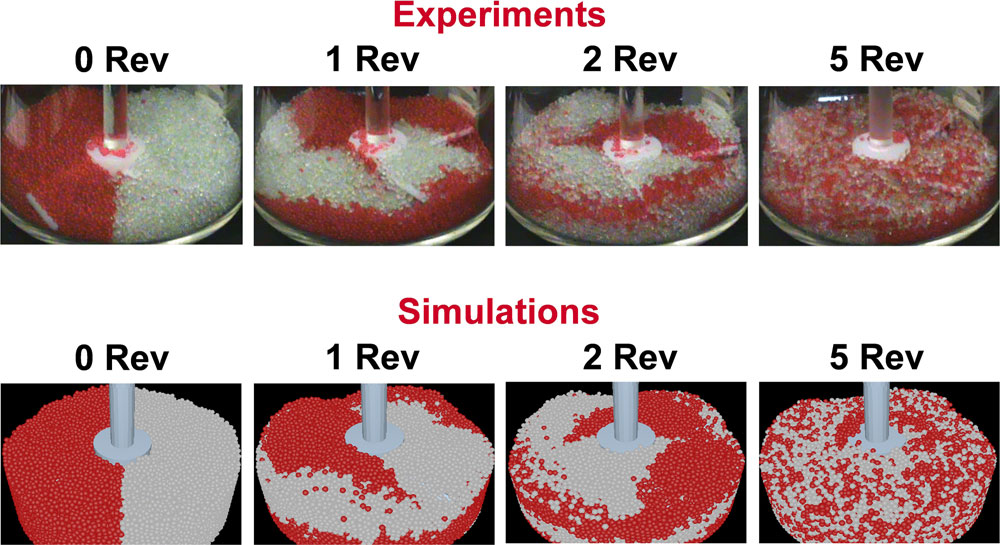
\includegraphics[width=0.65\textwidth]{images/drug_production.png}
	\end{center}
	% {\centerline{\includegraphics[scale=#2]{#1}}}
	% \vspace{-0.2cm}
	\label{fig:bidimensional_simulation}
	\source{\alert{Citar fonte}}
	% \vspace{-1cm}
\end{figure}

Além disso, da hipótese de que as rotações ocorrem apenas em torno do eixo \(\zAxis\) segue que o torque resultante possui apenas componentes nessa direção, isto é,
\begin{equation*}
	\resultingTorque = \torqueScalar\cdot \zUnit,
\end{equation*}
com \(\torqueScalar\in\real\).

Com isso, a equação \eqref{eq:motion_second} fica simplesmente
\begin{equation*}
	\torqueScalar = \zzMomentOfInertia\cdot\deriv{2}{\orientationScalar},
\end{equation*}
em que \(\zzMomentOfInertia\) é o momento de inércia escalar da partícula com relação ao eixo \(\zAxis\). Essa última equação se torna, então, a equação de movimento rotacional para partículas em simulações em duas dimensões.

Uma situação um pouco mais geral é que a direção da velocidade angular seja apenas constante, não necessariamente a do eixo \(\zAxis\), mas sim a de um eixo qualquer \(\zAxis^\prime\). Nesse caso, existe uma nova base \(\basis^\prime = \explicitVector{\xUnit^\prime}{\yUnit^\prime}{\zUnit^\prime}\) contendo os versores dos eixos \(\xAxis^\prime\yAxis^\prime\zAxis^\prime\) que satisfaz
\begin{equation*}
	\angularVelocity = \angularVelocityScalar\cdot\zUnit^\prime,
\end{equation*}
e, analogamente ao caso anterior, uma função de orientação \(\orientationScalar\) tal que
\begin{gather*}
	\angularVelocity = \deriv{1}{\orientationScalar}\cdot\zUnit^\prime, \\
	\angularAcceleration = \deriv{2}{\orientationScalar}\cdot\zUnit^\prime.
\end{gather*}

Novamente, a hipótese de direção de rotação constante implica que é possível escrever
\begin{equation*}
	\resultingTorque = \torqueScalar\cdot\zUnit^\prime,
\end{equation*}
e assim se obtém a equação
\begin{equation*}
	\torqueScalar = \zzMomentOfInertia^\prime\cdot\deriv{2}{\orientationScalar}.
\end{equation*}

Para a solução dessa equação, porém, ainda é necessária a determinação do valor de \(\zzMomentOfInertia^\prime\). Isso pode ser feito como sugere \citeonline{bib:dynamics_of_multibody_systems}, calculando-se a matriz de rotação \(\rotationMatrix\) que transforma as coordenadas de vetores definidos na base \(\basis\) em coordenadas definidas no sistema \(\xAxis^\prime\yAxis^\prime\zAxis^\prime\), na base \(\basis^\prime\), e obtendo
\begin{equation*}
	\matrixOfInertia^\prime =
	\begin{pmatrix}
		\xxMomentOfInertia^\prime & \xyMomentOfInertia^\prime & \xzMomentOfInertia^\prime \\
		\yxMomentOfInertia^\prime & \yyMomentOfInertia^\prime & \yzMomentOfInertia^\prime \\
		\zxMomentOfInertia^\prime & \zyMomentOfInertia^\prime & \zzMomentOfInertia^\prime
	\end{pmatrix}
	=
	\rotationMatrix\cdot \matrixOfInertia \cdot \transpose{\rotationMatrix}.
\end{equation*}

Embora tenda-se a evitar multiplicações matriciais, esse cálculo pode ser feito apenas uma vez, no início da simulação, desde que se saiba a priori a direção da rotação.

\subsubsection{Rotação de Partículas Esféricas} \label{subsubsec:rotation_of_spherical_particles}

Segundo \citeonline{bib:dynamics_of_multibody_systems}, para partículas esféricas, \textit{todas} as direções são uma direções principais. Sendo assim, o sistema de equações \eqref{eq:motion_second_system} é válido em qualquer sistema de eixos. Mais ainda, em função da simetria da partícula, ocorre que \(\momentOfInertia_1 = \momentOfInertia_2 = \momentOfInertia_3\). Ao se definir \(\momentOfInertia \eqdef \momentOfInertia_1\), obtém-se
\begin{equation*}
	\left\lbrace
	\begin{array}{l}
		\momentOfInertia\deriv{1}{\angularVelocityScalar_1} = \torqueScalar_1 \\
		\momentOfInertia\deriv{1}{\angularVelocityScalar_2} = \torqueScalar_2 \\
		\momentOfInertia\deriv{1}{\angularVelocityScalar_3} = \torqueScalar_3
	\end{array}
	\right.
	,
\end{equation*}
ou ainda
\begin{equation} \label{eq:rotation_spherical_particle}
	\resultingTorque = \momentOfInertia\cdot\angularAcceleration,
\end{equation}
e, com isso, a equação diferencial para o movimento de rotação está pronta para simulações tridimensionais de partículas esféricas.

\subsubsection{Rotação Geral em Três Dimensões} \label{subsubsec:general_rotation}

Para simulações em três dimensões com partículas não esféricas, utiliza-se o sistema de equações \eqref{eq:motion_second_system}. A solução do sistema, porém, não é trivial já que as equações são dadas em termos das direções principais da partícula.

As direções principais de uma partícula são dadas pela base ortonormal \(\principal{\basis} = \explicitVector{\principal{\xUnit}}{\principal{\yUnit}}{\principal{\zUnit}}\) cujos versores são autovetores da matriz de momento de inércia. A importância dessa base se dá pelo fato de que a matriz de momento de inércia se torna diagonal quando escrita em termos de seus vetores.

Entretanto, em virtude do caráter dinâmico dos sistemas de partículas, as direções principais dos elementos são funções do tempo: \(\principal{\basis} \equiv \principal{\basis}\pqty{t}\). Uma \textit{parametrização} para a orientação é qualquer conjunto de coordenadas \(\orientation\) que defina, equivalentemente, as direções principais. Diversas parametrizações já foram propostas, como mostrado no \autoref{app:three_dimensional_rotation}.

Com a parametrização \(\orientation\), sempre é possível obter os eixos principais através de uma transformação inversível:
\begin{equation*}
	\principal{\basis}\pqty{t} \leftrightarrow \orientation\pqty{t},
\end{equation*}
e, com isso, determina-se uma matriz de rotação \(\orientationRotationMatrix\) que transforma vetores da base de eixos locais na base das direções principais da partícula.

Ainda, com os eixos principais dados em função de \(\orientation\), a velocidade angular e suas derivadas podem ser escritas a partir da parametrização e suas derivadas:
\begin{gather*}
	\angularVelocity \equiv \angularVelocity\pqty{\orientation, \deriv{1}{\orientation}}, \\
	\deriv{1}{\angularVelocity} \equiv \deriv{1}{\angularVelocity}\pqty{\orientation, \deriv{1}{\orientation}, \deriv{2}{\orientation}}, \\
	\vdots \\
	\deriv{\taylorOrder}{\angularVelocity} \equiv \deriv{\taylorOrder}{\angularVelocity}\pqty{\orientation, \deriv{1}{\orientation}, \dots, \deriv{\taylorOrder+1}{\orientation}}.
\end{gather*}

Essas relações são inversíveis, e então é possível obter
\begin{gather*}
	\deriv{1}{\orientation} \equiv \deriv{1}{\orientation}\pqty{\orientation, \angularVelocity} \\
	\deriv{2}{\orientation} \equiv \deriv{2}{\orientation}\pqty{\orientation, \angularVelocity, \deriv{1}{\angularVelocity}} \\
	\vdots \\
	\deriv{\taylorOrder+1}{\orientation} \equiv \deriv{\taylorOrder+1}{\orientation}\pqty{\orientation, \angularVelocity, \dots, \deriv{\taylorOrder}{\angularVelocity}}
\end{gather*}

Assim, com a parametrização \(\orientation\), define-se toda a cinemática da rotação da partícula. Mais ainda, devido à equivalência entre o sistema de eixos principais e a parametrização, vetores definidos com relação ao sistema de eixos locais podem ser escritos em termos das direções principais. Isso significa que
\begin{equation*}
	\principal{\resultingTorque} \equiv \principal{\resultingTorque}\pqty{\resultingTorque, \orientation}.
\end{equation*}

Como resultado dessas considerações, o sistema de equações \eqref{eq:motion_second_system} transforma-se em uma equação diferencial da forma
\begin{equation} \label{eq:diff_equation_orientation_parametrization}
	\deriv{2}{\orientation} = \eqFor{\orientation}\pqty{\resultingTorque, \orientation, \deriv{1}{\orientation}}.
\end{equation}

A função \(\eqFor{\orientation}\) representa a dependência de \(\deriv{2}{\orientation}\) com relação a \(\resultingTorque\), \(\orientation\) e \(\deriv{1}{\orientation}\), e seu formato depende da definição da parametrização e da expressão para o torque resultante em função das variáveis do problema.

\subsection{Solução das Equações de Movimento} \label{subsec:motion_equations_solution}

Para a determinação do comportamento do sistema, é necessária a obtenção das soluções para as equações \eqref{eq:motion_first} e \eqref{eq:motion_second}. Isso exige  o cálculo da força e do torque resultantes sobre cada partícula e a consequente resolução da equação. 

O cálculo das forças e dos torques geralmente leva em conta \textit{modelos de interação}. Cada modelo determina uma parcela do vetor força ou torque resultante a partir de parâmetros de material, da posição, da velocidade, da orientação e da velocidade angular das partículas. Na \autoref{sec:collision_force_models}, são apresentados alguns desses modelos. Os vetores resultantes são então a soma de todas as parcelas.
 
Com os vetores força e torque resultantes, as equações diferenciais do movimento ficam bem determinadas. Resta a escolha de procedimentos para a resolução dessas equações, algoritmos chamados de \textit{métodos de integração} que, dadas duas partículas no instante \(t\) e as equações de movimento, sejam capazes de calcular as coordenadas e as propriedades dessas partículas em um instante futuro \(t+\Dt\).  
 
As principais características consideradas para a escolha de um método de solução das equações diferenciais são a exatidão, a estabilidade e o custo computacional. Neste trabalho, é utilizado o algoritmo de Gear, descrito na \autoref{sec:gear_integration_scheme}. A motivação para seu uso é que, como indicado na \autoref{sec:neighborhood}, o principal custo computacional dos métodos de elementos discretos advém do cômputo das forças em cada instante de tempo. O método de Gear necessita de apenas uma avaliação das interações por passo de tempo, o que representa uma eficiência máxima nesse sentido. A estabilidade do algoritmo ainda dispensa iterações dentro de cada passo de tempo, reduzindo, mais uma vez, o custo computacional. Outros algoritmos de integração são o método baseado em pontos centrais \textit{leapfrog}, os métodos de Verlet e os de Runge-Kutta \cite{bib:sampaio}.
 
De uma simulação, é possível extrair diversas informações. Alguns dos principais resultados que se buscam obter são a trajetória das partículas, o carregamento ou a pressão sobre determinada superfície, o coeficiente de restituição resultante das colisões, tempo para esvaziamento de um reservatório, entre outros.

O procedimento de se calcularem as forças e torques e, posteriormente, resolverem-se as equações diferenciais é conhecido como \textit{simulação baseada em forças}. Alternativamente a esse método, é possível executarem-se \textit{simulações orientadas a eventos}. Nessas simulações, apenas o coeficiente de restituição é considerado na colisão entre as partículas. Esse técnica está fora do escopo desse trabalho, mas pode ser encontrada com mais detalhes em \citeonline{bib:computational_granular_dynamics}.

\section{Modelos de Força de Colisão} \label{sec:collision_force_models}

Dentre as interações entre partículas do sistema, as mais comumente encontradas são as forças de colisão que surgem durante o seu contato. Os modelos de força têm o papel de atribuir, para cada par de partículas, uma componente de força \(\force\) e uma componente de torque \(\torque\).

Seguindo a notação apresentada na \autoref{sec:particle_systems}, denota-se por \(\forceji\) a componente de força aplicada pela partícula \(\particlej\) sobre a partícula \(\particlei\), e por \(\torqueji\) a componente de torque correspondente definida no sistema de eixos centrado na partícula \(\particlei\).

Os modelos de colisão mais simples são aqueles que ocorrem entre partículas esféricas ou entre uma partícula esférica e uma parede plana. Nesta seção, são apresentados alguns dos parâmetros geralmente utilizados na determinação de forças e torques e alguns dos principais modelos considerados, segundo \citeonline{bib:computational_granular_dynamics}. 

\subsection{Parâmetros de Cálculo} \label{subsec:collision_parameters}

Os principais parâmetros considerados para o cálculo das forças de colisão são a geometria das partículas, as suas propriedades físicas, a velocidade relativa no ponto de contato e a \textit{superposição}. Esses parâmetros, representados graficamente na figura \ref{fig:collision_parameters}, descrevem as condições em que a colisão ocorre, e assim determinam as componentes de força.

\begin{figure}[h]
	\caption{Parâmetros de Cálculo na Colisão entre Elementos}
	% \vspace{-0.5cm}
	\begin{center}
		\alert{Colocar figura aqui}
		% 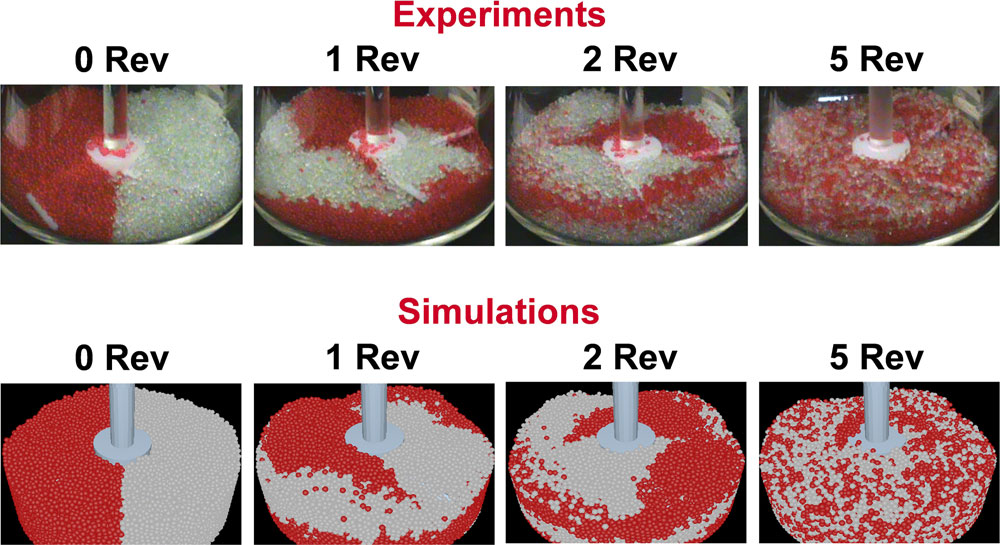
\includegraphics[width=0.65\textwidth]{images/drug_production.png}
	\end{center}
	% {\centerline{\includegraphics[scale=#2]{#1}}}
	% \vspace{-0.2cm}
	\label{fig:collision_parameters}
	\source{\alert{Citar fonte}}
	% \vspace{-1cm}
\end{figure}

\subsubsection*{Superposição} 

No Método de Elementos Discretos, os elementos são consideradas corpos rígidos. Sendo assim, quando ocorre contato entre dois elementos, não ocorre deformação, mas, sim, uma superposição ou penetração.

A medida da penetração pode variar dependendo dos tipos de elementos considerados. Para corpos com geometrias arbitrárias, pode ser necessária a medição do volume sobreposto. Entretanto, para um par de partículas esféricas ou um par formado por uma esfera e uma parede plana, é suficiente definir-se a superposição linearmente, como na figura \ref{fig:collision_parameters}.

Sendo \(\particlei\) e \(\particlej\) duas partículas esféricas distintas, pode-se definir a distância entre seus centros como 
\begin{equation*}
	\distanceij = \norm{\positionj - \positioni}.
\end{equation*}

Denotando-se por \(\radiusi\) e \(\radiusj\) os raios das partículas \(\particlei\) e \(\particlej\), ocorre que há superposição se, e somente se, \(\radiusi + \radiusj > \distanceij\). Nesse caso, a superposição \(\overlapij\) entre os elementos é dada por \(\overlapij = \radiusi + \radiusj - \distanceij\).

Caso a distância entre os centros das partículas seja maior que a soma de seus raios, a superposição é nula. Com isso, pode-se definir a superposição entre as partículas \(\particlei\) e \(\particlej\) como
\begin{equation} \label{eq:overlap}
	\overlapij = \max\Bqty{\radiusi + \radiusj - \distanceij, 0}.
\end{equation}

A simples diferenciação da equação \eqref{eq:overlap} com relação ao tempo resulta na derivada da superposição:
\begin{equation} \label{eq:spherical_particle_overlap_derivative}
	\overlapDerivativeij =
	\left\lbrace
	\begin{array}{cl}
		- \dfrac{\innerProduct{\positionj - \positioni}{\velocityj - \velocityi}}{\norm{\positionj - \positioni}},
		& \text{se } \overlapij > 0 \\
		0, & \text{se } \overlapij = 0
	\end{array}
	\right.
	,
\end{equation}
em que \(\innerProduct{\dummy}{\dummy}\) representa o produto interno entre vetores.

Para o caso do contato entre esfera e parede plana, consideram-se \(\particlei\) uma partícula esférica e \(\elementj\) um elemento plano fixo no espaço. Sejam \(\planeOriginj\) um ponto nesse plano e \(\planeNormalVersorj\) um versor normal a ele. A distância do centro de \(\particlei\) ao plano é dada por
\begin{equation*}
	\distanceij = \abs{\innerProduct{\positioni - \planeOriginj}{\planeNormalVersorj}}.
\end{equation*}

Assim, a sobreposição entre \(\particlei\) e \(\elementj\) fica
\begin{equation*}
	\overlapij = \max\Bqty{\radiusi - \distanceij, 0},
\end{equation*}
e sua derivada,
\begin{equation*}
	\overlapDerivativeij =
	\left\lbrace
	\begin{array}{cl}
		- \innerProduct{\velocityi}{\planeNormalVersorj}, & \text{se } \overlapij > 0 \text{ e } \innerProduct{\positioni - \planeOriginj}{\planeNormalVersorj} > 0\\
		\innerProduct{\velocityi}{\planeNormalVersorj}, & \text{se } \overlapij > 0 \text{ e } \innerProduct{\positioni - \planeOriginj}{\planeNormalVersorj} < 0\\
		0, & \text{se } \overlapij = 0
	\end{array}
	\right.
	.
\end{equation*}

\subsubsection*{Versor Normal}

Sendo \(\particlei\) e \(\particlej\) duas partículas esféricas, o versor normal que aponta de \(\particlei\) para \(\particlej\) é dado por
\begin{equation*}
	\normalVersorij = \normalized{\positionj - \positioni},
\end{equation*}
e é fácil ver que \(\normalVersorij = - \normalVersorji\).

Com isso, a derivada da superposição entre partículas esféricas pode ser calculada, equivalentemente à equação \eqref{eq:spherical_particle_overlap_derivative}, como
\begin{equation} \label{eq:particle_wall_overlap_derivative}
	\overlapDerivativeij =
	\left\lbrace
	\begin{array}{cl}
		- \innerProduct{\velocityj-\velocityi}{\normalVersorij}, & \text{se } \overlapij > 0 \\
		0, & \text{se } \overlapij = 0
	\end{array}
	\right.
	.
\end{equation}


Já para o caso de um elemento plano fixo \(\elementj\), o versor normal \(\normalVersorji\) é idêntico ao versor normal ao plano, isto é,
\begin{equation*}
	\normalVersorji = \planeNormalVersorj,
\end{equation*}
e \(\normalVersorij = - \normalVersorji\).

Em ambos os casos, é possível construir-se, a partir do centro da partícula \(i\), a reta normal \(\normalLineij\) da colisão entre \(i\) e \(j\) como o espaço gerado por \(\normalVersorij\):
\begin{equation*}
	\normalLineij = \set{\positioni + \radialVectorScalar\cdot\normalVersorij\suchThat\radialVectorScalar\in\real}.
\end{equation*}

\subsubsection*{Ponto de Contato}

Tanto na colisão entre partículas esféricas quanto na colisão entre partícula esférica e parede plana, existe um único plano, denominado de \textit{plano de contato} e denotado por \(\contactPlaneij\), que contém todos os pontos de interseção entre as superfícies dos colidentes, como mostra a figura \ref{fig:contact_point}.

\begin{figure}[h]
	\caption{Plano e ponto de contato entre dois elementos colidentes}
	% \vspace{-0.5cm}
	\begin{center}
		\alert{Colocar figura aqui}
		% 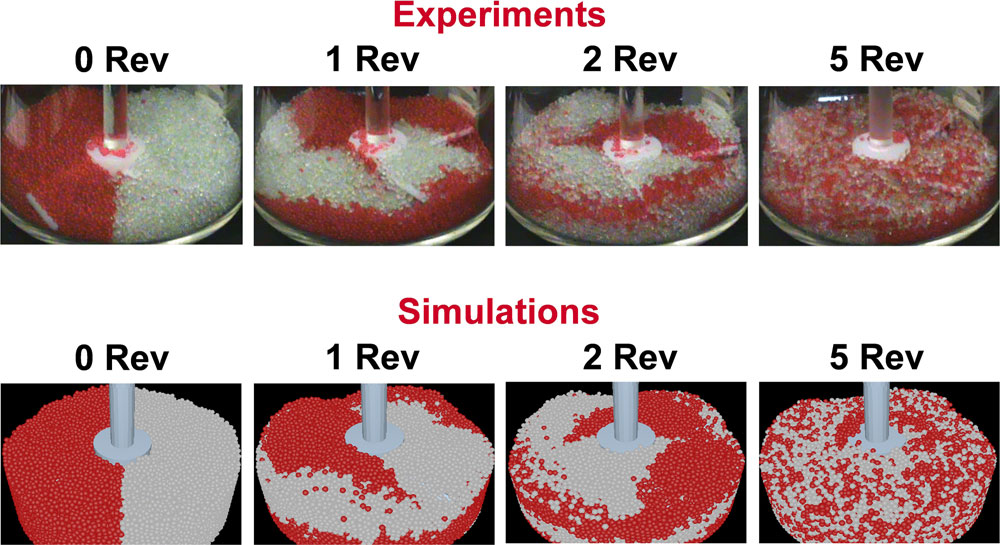
\includegraphics[width=0.65\textwidth]{images/drug_production.png}
	\end{center}
	% {\centerline{\includegraphics[scale=#2]{#1}}}
	% \vspace{-0.2cm}
	\label{fig:contact_point}
	\source{\alert{Citar fonte}}
	% \vspace{-1cm}
\end{figure}

O ponto de contato efetivo \(\contactPointij\) entre os elementos \(i\) e \(j\) é dado pela interseção entre o plano de contato e a reta normal \(\normalLineij\). Vetorialmente, o contato é representado pela posição \(\vectorFromPoints{\originPoint}{\contactPointij}\).

Esse ponto também pode ser representado pelo vetor radial \(\contactVectorij = \contactRadiusij\cdot\normalVersorij\) como
\begin{equation} \label{eq:contact_point}
	\vectorFromPoints{\originPoint}{\contactPointij} = \positioni + \contactVectorij.
\end{equation}

Para duas partículas esféricas, a geometria do contato é tal como mostrado na figura \ref{fig:contact_geometry}. Segue então do teorema de Pitágoras que
\begin{equation*}
	\radiusi^2 - \contactRadiusij^2 = \radiusj^2 - \contactRadiusji^2.
\end{equation*}

\begin{figure}[h]
	\caption{Geometria do Contato para Partículas Esféricas}
	% \vspace{-0.5cm}
	\begin{center}
		\alert{Colocar figura aqui}
		% 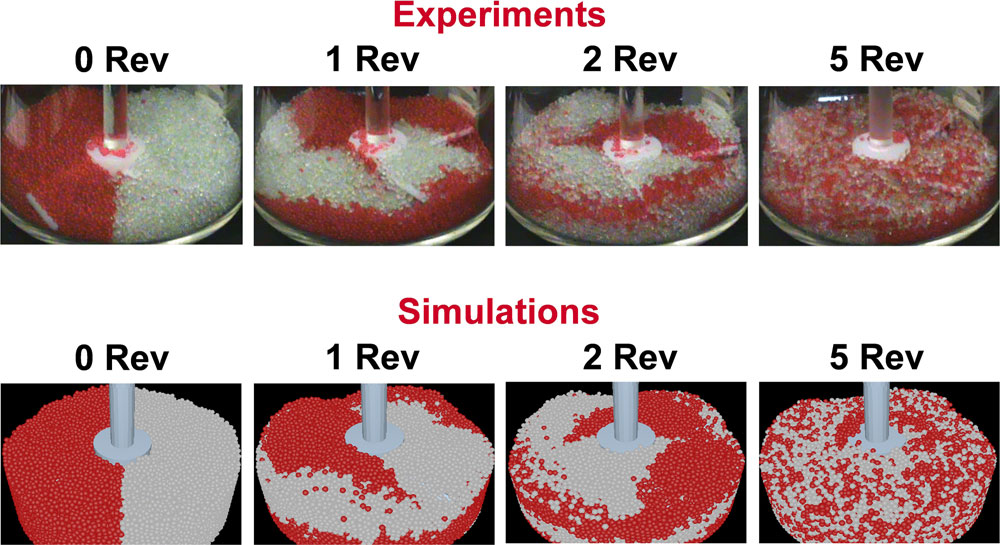
\includegraphics[width=0.65\textwidth]{images/drug_production.png}
	\end{center}
	% {\centerline{\includegraphics[scale=#2]{#1}}}
	% \vspace{-0.2cm}
	\label{fig:contact_geometry}
	\source{\alert{Citar fonte}}
	% \vspace{-1cm}
\end{figure}

Além disso,
\begin{equation*}
	\contactRadiusij + \contactRadiusji = \distanceij,
\end{equation*}
e então, ao se combinarem essas duas equações,
\begin{equation} \label{eq:contact_radius}
	\contactRadiusij = \dfrac{\radiusi^2 - \radiusj^2 + \distanceij^2}{2\cdot\distanceij}.
\end{equation}

Com as equações \eqref{eq:contact_point} e \eqref{eq:contact_radius}, o ponto de contato fica bem determinado.

A situação se simplifica para a colisão entre uma partícula esférica e um elemento plano, já que ocorre que
\begin{equation*}
	\contactRadiusij = \distanceij.
\end{equation*}

Em ambos os casos, com a definição do vetor radial \(\contactVectorij\), a componente de força \(\forceji\) está associada a uma componente de torque \(\torqueji\) dada por
\begin{equation*}
	\torqueji = \contactVectorij\cross\forceji
\end{equation*}

\subsubsection*{Velocidade Relativa no Ponto de Contato}

A velocidade relativa no ponto de contato é o principal parâmetro cinemático na determinação da força tangencial que ocorre entre dois elementos. A velocidade do elemento \(j\) relativa ao elemento \(i\) no ponto de contato é denotada por \(\relativeVelocityContactPointij\).

O cálculo dessa velocidade leva em consideração o fato de que, no ponto de contato \(\contactPointij\), estão superpostos dois pontos: um ponto \(\contactPointi\) pertencente à partícula \(i\), e um ponto \(\contactPointj\) que pertence ao elemento \(j\). Cada um desses pontos move-se juntamente com o elemento correspondente e, por ocasião do contato, os dois acabam por se encontrar. Isso é representado na figura \ref{fig:relative_velocity}.

\begin{figure}[h]
	\caption{Velocidade relativa no ponto de contato}
	% \vspace{-0.5cm}
	\begin{center}
		\alert{Colocar figura aqui}
		% 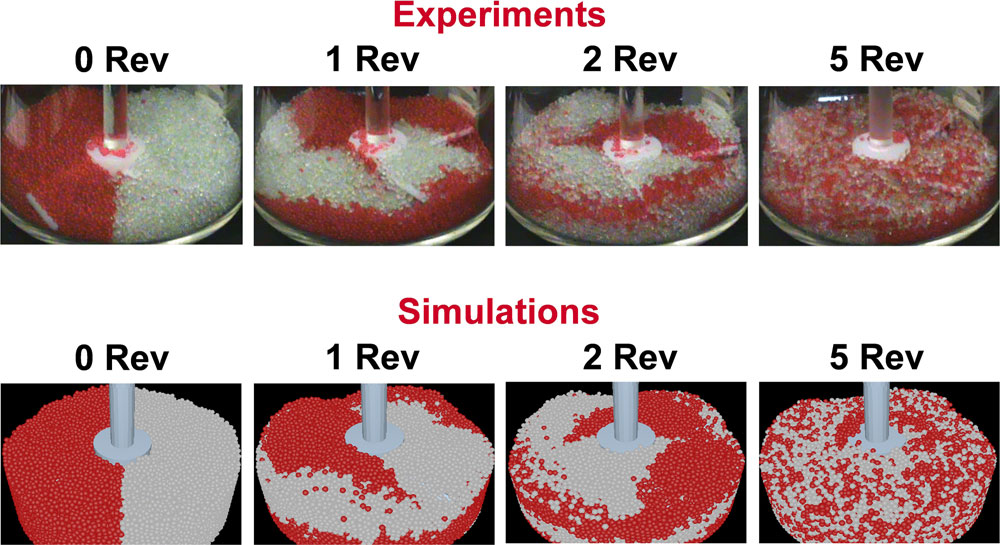
\includegraphics[width=0.65\textwidth]{images/drug_production.png}
	\end{center}
	% {\centerline{\includegraphics[scale=#2]{#1}}}
	% \vspace{-0.2cm}
	\label{fig:relative_velocity}
	\source{\alert{Citar fonte}}
	% \vspace{-1cm}
\end{figure}

Como esses pontos movem-se no espaço, os vetores \(\vectorFromPoints{\originPoint}{\contactPointi}\) e \(\vectorFromPoints{\originPoint}{\contactPointj}\) não são constantes, mas, sim, funções do tempo. A velocidade \(\relativeVelocityContactPointij\) é então definida como a velocidade relativa entre esses dois vetores:
\begin{equation*}
	\relativeVelocityContactPointij = \dv{t}(\vectorFromPoints{\originPoint}{\contactPointj} - \vectorFromPoints{\originPoint}{\contactPointi}).
\end{equation*}

De acordo com \citeonline[p. 25]{bib:dynamics_of_multibody_systems}, e usando o fato de que os pontos \(\contactPointi\) e \(\contactPointj\) são fixos nos elementos a que pertencem (ou seja, os pontos têm velocidade relativa nula com relação aos seus respectivos corpos), é possível escrever
\begin{gather*}
	\dv{t}(\vectorFromPoints{\originPoint}{\contactPointi}) = \velocityi + \angularVelocityi\cross\contactVectorij, \\
	\dv{t}(\vectorFromPoints{\originPoint}{\contactPointj}) = \velocityj + \angularVelocityj\cross\contactVectorji.
\end{gather*}

Com isso, obtém-se
\begin{equation*}
	\relativeVelocityContactPointij = \pqty{\velocityj - \velocityi} + \pqty{\angularVelocityj\cross\contactVectorji - \angularVelocityi\cross\contactVectorij}.
\end{equation*}

Nota-se dessa equação que
\begin{equation} \label{eq:antisymmetry_relative_velocity}
	\relativeVelocityContactPointji = - \relativeVelocityContactPointij.
\end{equation}

A velocidade normal de \(j\) relativa ao elemento \(i\) é a projeção de \(\relativeVelocityContactPointij\) na direção de \(\normalVersorij\):
\begin{equation} \label{eq:relative_normal_velocity}
	\begin{array}{rl}
		\relativeNormalVelocityij & = \innerProduct{\relativeVelocityContactPointij}{\normalVersorij}\cdot\normalVersorij \\
		& = \relativeNormalVelocityScalarij\cdot\normalVersorij.
	\end{array}
\end{equation}

Percebe-se, em consequência das equações \eqref{eq:spherical_particle_overlap_derivative}, \eqref{eq:particle_wall_overlap_derivative} e \eqref{eq:relative_normal_velocity}, que, tanto para a colisão entre partículas esféricas quanto para a colisão entre uma esfera e uma parede plana, ocorre que
\begin{equation} \label{eq:overlap_derivative_and_normal_relative_velocity}
	\overlapDerivativeij = - \relativeNormalVelocityScalarij.
\end{equation}

Por sua vez, velocidade tangencial de \(j\) relativa ao elemento \(i\) é simplesmente a correspondente velocidade relativa sem a componente na direção normal:
\begin{equation*}
	\relativeTangentialVelocityij = \relativeVelocityContactPointij - \innerProduct{\relativeVelocityContactPointij}{\normalVersorij}\cdot\normalVersorij.
\end{equation*}

As simplificações que se fazem no caso em que o elemento \(j\) é uma parede plana são que 
\begin{gather*}
	\velocityj = \nullVector, \\
	\angularVelocityj = \nullVector,
\end{gather*}
do que segue que
\begin{equation} \label{eq:sphere_plane_relative_velocity}
	\relativeVelocityContactPointij = - \velocityi - \angularVelocityi\cross\contactVectorij.
\end{equation}

\subsubsection*{Versor Tangencial}

Com a velocidade tangencial determinada, é possível definir-se o versor tangencial \(\tangentialVersorij\) como
\begin{equation*}
	\tangentialVersorij = \normalized{\relativeTangentialVelocityij},
\end{equation*}
e então escrever
\begin{equation*}
	\relativeTangentialVelocityij = \relativeTangentialVelocityScalarij\cdot \tangentialVersorij.
\end{equation*}

Para o caso em que \(\relativeTangentialVelocityij = \nullVector\), não é necessário calcular-se o versor tangencial pois, nessa situação, as forças tangenciais são sempre nulas, de acordo com os modelos de interação.

\subsubsection*{Coeficiente de Restituição} 

A determinação do coeficiente de restituição tem a vantagem de poder simplificar e reduzir o tempo de simulação em simulações orientadas a eventos, mas também pode ser usada para a validação de métodos numéricos baseados no cálculo das forças, que são o foco deste trabalho.

Para cada par de elementos, o coeficiente de restituição relaciona o estado posterior ao choque ao estado anterior. Escrevendo a velocidade do elemento \(j\) relativa ao \(i\) imediatamente antes da colisão como \(\beforeCollision{\relativeVelocityContactPointij}\), e a velocidade correspondente no final da colisão como \(\afterCollision{\relativeVelocityContactPointij}\), define-se o coeficiente de restituição na direção normal \(\normalCoefficientOfRestitutionij\) através da equação
\begin{equation*}
	\afterCollision{\relativeNormalVelocityScalarij} = - \normalCoefficientOfRestitutionij\cdot\beforeCollision{\relativeNormalVelocityScalarij}.
\end{equation*}

De acordo com \citeonline{bib:computational_granular_dynamics}, a seguinte desigualdade é sempre satisfeita:
\begin{equation*}
	0 \leq \normalCoefficientOfRestitutionij \leq 1.
\end{equation*}

Formas analíticas para o coeficiente de restituição podem ser obtidas através da integração das equações diferenciais, dependendo dos modelos de interação considerados. Em função da complexidade do modelo, pode ser muito difícil, ou mesmo impossível, de se obter uma forma fechada para esse coeficiente. Outras maneiras de se determinar seu valor são o uso de simulações numéricas e a experimentação, em que se busca correlacioná-lo com as demais grandezas do problema.

De forma geral, o valor desse coeficiente depende de parâmetros de material e da velocidade relativa entre as partículas. Segundo \citeonline{bib:computational_granular_dynamics}, coeficientes de restituição constantes (independentes da velocidade relativa) estão em desacordo com resultados experimentais e com o importante modelo de partículas viscoelásticas. Entretanto coeficientes constantes formam a base para diversas teorias e podem ser bastante úteis para a validação de métodos numéricos.

É possível ainda definir-se um coeficiente de restituição tangencial \(\tangentialCoefficientOfRestitutionij\) conforme \citeonline{bib:computational_granular_dynamics}, mas esse coeficiente não é considerado neste trabalho.

Feitas essas considerações, os principais parâmetros para o cálculo das forças e torques de colisão estão bem definidos. Nas seções \ref{subsec:normal_force_models} e \ref{subsec:tangential_force_models} são apresentados alguns dos modelos de força mais adotados e que se utilizam desses parâmetros.

\subsection{Modelos de Força Normal} \label{subsec:normal_force_models}

Nesta seção, são apresentados os dois principais modelos de força normal utilizados nas simulações de elementos discretos. Ambos os modelos buscam determinar
\begin{equation*}
	\normalForceji = \normalForceScalarji\cdot\normalVersorji.
\end{equation*}

\subsubsection*{Modelo de Amortecedor Linear}

O modelo de amortecedor linear é um dos modelos mais simples que se adotam para a colisão de partículas. Esse modelo pode ser representado esquematicamente como na figura \ref{fig:linear_dashpot_force}.

\begin{figure}[h]
	\caption{Representação do modelo de amortecimento linear}
	% \vspace{-0.5cm}
	\begin{center}
		\alert{Colocar figura aqui}
		% 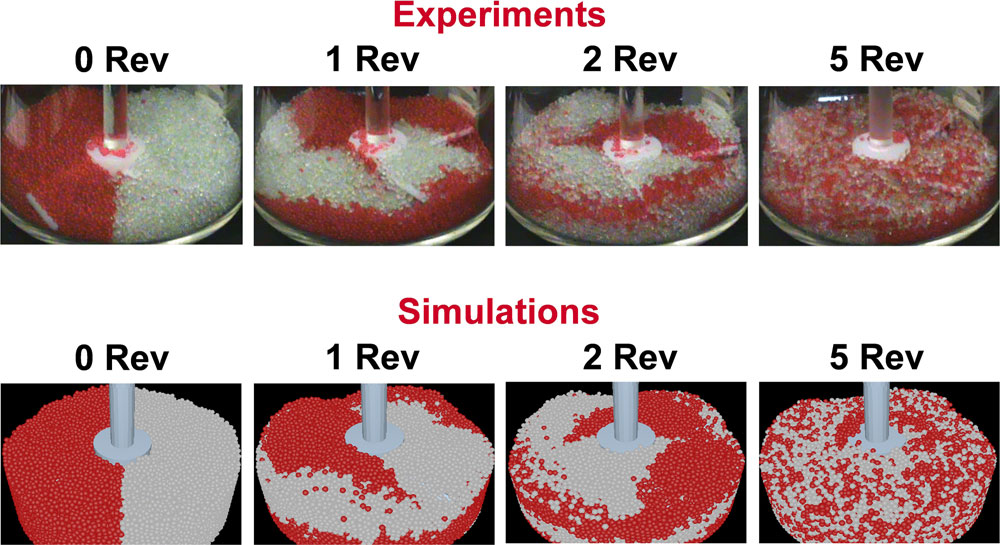
\includegraphics[width=0.65\textwidth]{images/drug_production.png}
	\end{center}
	% {\centerline{\includegraphics[scale=#2]{#1}}}
	% \vspace{-0.2cm}
	\label{fig:linear_dashpot_force}
	\source{\alert{Citar fonte}}
	% \vspace{-1cm}
\end{figure}

A equação para a força normal dada por esse modelo é
\begin{equation} \label{eq:linear_dashpot_force}
	\normalForceScalarji = \elasticModulusij\cdot\overlapij + \normalDampingConstantij\cdot\overlapDerivativeij,
\end{equation}
em que:
\begin{itemize}
	\item \(\elasticModulusij\) é a constante elástica efetiva para o par de partículas \(i\) e \(j\). Esse valor efetivo é calculado pela associação em série de molas elásticas, do que resulta que
	\begin{equation*}
		\elasticModulusij = \pqty{\dfrac{1}{\elasticModulusi} + \dfrac{1}{\elasticModulusj}}^{-1},
	\end{equation*}
	sendo \(\elasticModulusi\) e \(\elasticModulusj\) as constantes elásticas das partículas \(i\) e \(j\), respectivamente.

	A constante elástica representa a rigidez das partículas, sendo que elementos com maior constante elástica resistem mais à penetração. Essa constante é uma propriedade de material de cada partícula.

	\item \(\normalDampingConstantij\) é a constante de amortecimento efetiva para o par \(\pqty{i, j}\), calculada através da associação em série de amortecedores de constantes \(\normalDampingConstanti\) e \(\normalDampingConstantj\):
	\begin{equation*}
		\normalDampingConstantij = \pqty{\dfrac{1}{\normalDampingConstanti} + \dfrac{1}{\normalDampingConstantj}}^{-1}.
	\end{equation*}

	A constante de amortecimento corresponde à dissipação de energia na colisão. Maiores amortecimentos indicam maior perda de energia no choque. Essa constante é atribuída a cada partícula como se fosse uma propriedade de material. Essa atribuição, porém, muitas vezes não é possível, e se torna necessária a execução de experimentos para a determinação do valor dessa constante.
\end{itemize}

A partir da equação \eqref{eq:linear_dashpot_force} e da primeira equação de movimento \eqref{eq:motion_first}, é possível derivar-se uma expressão para o coeficiente de restituição na direção normal. Para um par de partículas esféricas, a massa efetiva é definida como
\begin{equation*}
	\massij = \pqty{\massi^{-1} + \massj^{-1}}^{-1},
\end{equation*}
e, para o caso em que a \(i\)-ésima partícula é esférica e a \(j\)-ésima representa uma parede plana,
\begin{equation*}
	\massij = \massi.
\end{equation*}

Com isso, o coeficiente de restituição normal do par de partículas fica, de acordo com \citeonline{bib:computational_granular_dynamics},
\begin{equation*}
	\normalCoefficientOfRestitutionij = \exp\pqty{
		\bigslant{
			-\dfrac{\pi\normalDampingConstantij}{2\massij}
		}{
			\sqrt{\dfrac{\elasticModulusij}{\massij} - \pqty{\dfrac{\normalDampingConstantij}{2\massij}}^2}
		}
	}.
\end{equation*}

Percebe-se dessa expressão que o modelo de amortecedor linear implica um coeficiente de restituição normal independente da velocidade relativa entre as partículas, o que não representa bem o comportamento real de sistemas, como afirmado na seção \ref{subsec:collision_parameters}. Entretanto, justamente devido à simplicidade da expressão, esse modelo é utilizado na teoria de gases granulares, em simulações de Dinâmica Molecular e na validação de métodos numéricos.

\subsubsection*{Modelo de Esferas Viscoelásticas}

Embora a equação \eqref{eq:linear_dashpot_force} represente de maneira simplificada a força entre duas partículas colidentes, ela captura os dois principais mecanismos de interação, que são o termo elástico, representado por \(\normalElasticForceji = \elasticModulusij\cdot\overlapij\), e o termo dissipativo, \(\normalDissipativeForceji = \normalDampingConstantij\cdot\overlapDerivativeij\).

O modelo para esferas viscoelásticas tem a finalidade de expressar de forma mais fidedigna esses dois termos.

\citeonline{bib:hertz1881} propôs primeiramente um modelo para a componente elástica da força, obtendo
\begin{equation*}
	\normalElasticForceji = \dfrac{4}{3}\effectiveNormalElasticij\sqrt{\effectiveRadiusij}\cdot\overlapij^{\sfrac{3}{2}},
\end{equation*}
sendo que:
\begin{itemize}
	\item \(\effectiveNormalElasticij\) é a constante elástica normal efetiva do par. Essa constante é definida por
		\begin{equation*}
			\effectiveNormalElasticij = \pqty{\dfrac{1-\poissoni^2}{\elasticModulusi} + \dfrac{1-\poissonj^2}{\elasticModulusj}}^{-1},
		\end{equation*}
		em que \(\poissoni\) e \(\poissonj\) são os coeficientes de Poisson das partículas \(i\) e \(j\), respectivamente.

	\item \(\effectiveRadiusij\) é o raio efetivo do par de partículas. Esse raio é definido como
		\begin{equation*}
			\effectiveRadiusij = \pqty{\radiusi^{-1} + \radiusj^{-1}}^{-1}.
		\end{equation*}
\end{itemize}

Esse modelo foi posteriormente estendido por \citeonline{bib:brilliantov1996} com a adição do termo dissipativo:
\begin{equation*}
	\normalDissipativeForceji = \dfrac{4}{3}\effectiveNormalElasticij\sqrt{\effectiveRadiusij}\cdot \normalDissipativeConstantij\overlapDerivativeij\sqrt{\overlapij},
\end{equation*}
em que
\begin{itemize}
	\item \(\normalDissipativeConstantij\) é a constante dissipativa efetiva do par. Essa constante é definida como a média aritmética das constantes dissipativas de cada partícula, isto é,
	\begin{equation*}
		\normalDissipativeConstantij = \dfrac{\normalDissipativeConstanti + \normalDissipativeConstantj}{2}.
	\end{equation*}

	De acordo com \citeonline{bib:computational_granular_dynamics}, não é possível relacionar a constante dissipativa a propriedades de material. Essa constante, porém, pode ser calculada em função do coeficiente de atrito entre as partículas, e este, por sua vez, pode ser determinado experimentalmente.
\end{itemize}

Com isso, a expressão para a força normal, segundo o modelo de esferas viscoelásticas, fica
\begin{equation*}
	\normalForceScalarji = \dfrac{4}{3}\effectiveNormalElasticij\sqrt{\effectiveRadiusij}\cdot\pqty{
		\overlapij^{\sfrac{3}{2}} + \normalDissipativeConstantij\overlapDerivativeij\sqrt{\overlapij}
	}.
\end{equation*}

O coeficiente de restituição normal, nesse caso, é uma função da velocidade normal relativa no início do choque. Esse valor se expressa na equação
\begin{equation*}
	\begin{array}{rl}
	\normalCoefficientOfRestitutionij\pqty{\beforeCollision{\relativeNormalVelocityScalarij}} & = 
	1
	+ C_1 \normalDissipativeConstantij\rho^{\sfrac{2}{5}}\pqty{\relativeNormalVelocityScalarij}^{\sfrac{1}{5}}
	+ C_2 \normalDissipativeConstantij^2 \rho^{\sfrac{4}{5}}\pqty{\relativeNormalVelocityScalarij}^{\sfrac{2}{5}}
	+ C_3 \normalDissipativeConstantij^3 \rho^{\sfrac{6}{5}}\pqty{\relativeNormalVelocityScalarij}^{\sfrac{3}{5}}
	+ \dotsb \\
	& \displaystyle = 1 + \sum_{m=1}^{+\infty} C_m \normalDissipativeConstantij^m \rho^{\sfrac{2m}{5}}\pqty{\relativeNormalVelocityScalarij}^{\sfrac{m}{5}},
	\end{array}
\end{equation*}
sendo que as constantes \(C_m\) são bem determinadas \cite[p. 143]{bib:computational_granular_dynamics} e
\begin{equation*}
	\rho \eqdef \dfrac{4\cdot\effectiveNormalElasticij}{3}\cdot\dfrac{\sqrt{\effectiveRadiusij}}{\massij}.
\end{equation*}

O modelo de esferas viscoelásticas se aproxima melhor dos resultados experimentais que o modelo de amortecedor linear, sendo por isso mais utilizado em simulações de sistemas reais \cite[p. 143]{bib:computational_granular_dynamics}.

\subsubsection*{Duração das Colisões}

Um problema que se encontra com a definição dos modelos de amortecedor linear e de esferas viscoelásticas é a inversão de sinal da força.

No início do choque, tanto a superposição quanto a sua derivada são positivas. Isso implica, de acordo com as expressões para a força, que ocorre repulsão entre as partículas. A penetração entre as partículas aumenta gradativamente até que, em determinado instante, atinge um valor máximo. Devido à força normal repulsiva, inicia-se o fenômeno de descompressão, em que as partículas se afastam. Nessa etapa, a derivada da superposição é negativa. É possível, dependendo dos parâmetros da simulação, que essa derivada negativa resulte em uma força normal \textit{atrativa}. Essa atração se inicia quando \(\overlapDerivativeij\) atinge um valor crítico \(\principal{\overlapDerivativeij}\), em que a força calculada é nula.

\begin{figure}[h]
	\caption{Representação da colisão entre partículas. Na primeira linha, a avaliação das forças segundo os modelos não corrigidos. Na segunda linha, a colisão com forças limitadas à repulsão.}
	% \vspace{-0.5cm}
	\begin{center}
		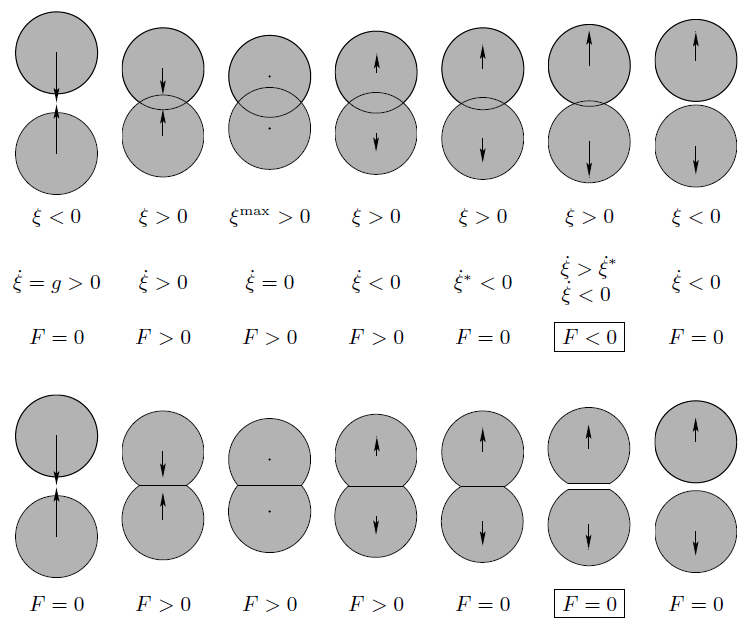
\includegraphics[width=0.9\textwidth]{images/mathematical_model/particle_attraction.PNG}
	\end{center}
	% {\centerline{\includegraphics[scale=#2]{#1}}}
	% \vspace{-0.2cm}
	\label{fig:particle_attraction}
	\source{\adapted{\citeonline[p. 22]{bib:computational_granular_dynamics}}}
	% \vspace{-1cm}
\end{figure}

No entanto a atração entre partículas geralmente não condiz com resultados experimentais. Uma das técnicas para eliminar esse fenômeno é limitarem-se inferiormente as forças calculadas. Esse artifício justifica-se pois, embora tenha sido feita a hipótese de que as partículas sejam corpos rígidos, partículas reais são deformáveis, e essa deformação pode ser suficiente para encerrar a colisão em um tempo anterior àquele considerado pelo modelo de partículas rígidas. Isso é representado na figura \ref{fig:particle_attraction}.

Para o amortecedor linear, isso significa que
\begin{equation*}
	\normalForceScalarji = \max\Bqty{\elasticModulusij\cdot\overlapij + \normalDampingConstantij\cdot\overlapDerivativeij, \,\, 0},
\end{equation*}
enquanto, para o modelo de esferas viscoelásticas, essa correção resulta em
\begin{equation*}
	\normalForceScalarji = \max\Bqty{\dfrac{4}{3}\effectiveNormalElasticij\sqrt{\effectiveRadiusij}\cdot\pqty{
		\overlapij^{\sfrac{3}{2}} + \normalDissipativeConstantij\overlapDerivativeij\sqrt{\overlapij}
	}, \,\, 0}.
\end{equation*}

Como consequência dessa mudança, o coeficiente de restituição normal tem seu valor alterado. \citeonline{bib:linear_dashpot_revisited} demonstram que, para o modelo de amortecedor linear, o coeficiente de restituição normal fica
\begin{equation*}
	\normalCoefficientOfRestitutionij = 
	\left\lbrace
		\def\arraystretch{1.8}
		\begin{array}{ll}
			\exp\bqty{-\dfrac{\betaij}{\omegaij}\pqty{\pi - \arctan\dfrac{2\betaij\omegaij}{\omegaij^2-\betaij^2}}}, & \text{se } \betaij < \dfrac{\omegazij}{\sqrt{2}} \\
			\exp\bqty{-\dfrac{\betaij}{\omegaij}\arctan\dfrac{2\betaij\omegaij}{\omegaij^2-\betaij^2}}, & \text{se } \betaij \in \bqty{\dfrac{\omegazij}{\sqrt{2}}, \omegazij} \\
			\exp\bqty{-\dfrac{\betaij}{\Omegaij} \ln\dfrac{\betaij + \Omegaij}{\betaij - \Omegaij}}, & \text{se } \betaij > \omegazij
		\end{array}
	\right.
	,
\end{equation*}
em que
\begin{equation*}
	\def\arraystretch{1.5}
	\begin{array}{cc}
		\omegazij = \bigslant{\effectiveNormalElasticij}{\massij}, &
		\betaij = \bigslant{\normalDampingConstantij}{\massij}, \\
		\omegaij = \sqrt{\pqty{\omegazij}^2 - \betaij^2}, &	\Omegaij = \sqrt{\betaij^2 - \pqty{\omegazij}^2}.
	\end{array}
\end{equation*}

\subsection{Modelos de Força Tangencial} \label{subsec:tangential_force_models}

Modelos para forças tangenciais, diferentemente dos modelos para forças normais, têm caráter intrinsecamente dinâmico, resistindo sempre ao movimento relativo entre as partículas. Esses modelos são responsáveis por fornecer um valor de força tangencial
\begin{equation*}
	\tangentialForceji = \tangentialForceScalarji\tangentialVersorji.
\end{equation*}

O fato de que essa força resiste ao movimento é representado pela desigualdade
\begin{equation*}
	\tangentialForceScalarji \leq 0.
\end{equation*}

Ainda, pela lei de Coulomb, a força tangencial não pode superar, em módulo, a força de atrito dinâmico 
\begin{equation*}
	\dynamicFrictionForceji = - \dynamicFrictionij\normalForceScalarji\cdot\tangentialVersorji,
\end{equation*}
em que \(\dynamicFrictionij\) é o coeficiente de atrito dinâmico entre o par de partículas \(\particlei\) e \(\particlej\). Disso segue a desigualdade
\begin{equation} \label{eq:coulomb_law}
	\tangentialForceScalarji \geq - \dynamicFrictionij\normalForceScalarji.
\end{equation}

Ao se determinar a força tangencial, a componente de torque \(\torqueji\) que a partícula \(j\) aplica sobre a \(i\) pode ser calculada como
\begin{equation*}
	\torqueji = \contactVectorij\cross\tangentialForceji
\end{equation*}

Nesta seção, são apresentados os dois principais modelos de força tangencial, de acordo com \citeonline{bib:computational_granular_dynamics}.

\subsubsection*{Modelo de Haff e Werner}

O modelo de Haff e Werner já foi aplicado com sucesso em diversas simulações. Esse modelo é o análogo tangencial do modelo de amortecedor linear para a força normal \cite{bib:computational_granular_dynamics}.

Para partículas esféricas, supondo que há contato, a equação \eqref{eq:overlap_derivative_and_normal_relative_velocity} sugere a analogia
\begin{equation*}
	\overlapDerivativeij \to \relativeTangentialVelocityScalarij
\end{equation*}

Além disso, devido ao caráter dinâmico da força tangencial, desconsideram-se componentes elásticas.

Com essas considerações e com a restrição da lei de Coulomb \eqref{eq:coulomb_law}, o análogo tangencial da equação \eqref{eq:linear_dashpot_force} fica
\begin{equation*}
	\tangentialForceScalarji = - \min\set{\tangentialDampingConstantij\cdot\relativeTangentialVelocityScalarij,\,\, \dynamicFrictionij\cdot\normalForceScalarji},
\end{equation*}
em que
\begin{itemize}
	\item \(\tangentialDampingConstantij\) é a constante de amortecimento tangencial efetiva do par \(i\) e \(j\). Essa constante pode ser obtida por uma associação em série de amortecedores de constantes \(\tangentialDampingConstanti\) e \(\tangentialDampingConstantj\), cada um pertencente a uma das partículas, como
	\begin{equation*}
		\tangentialDampingConstantij = \pqty{\dfrac{1}{\tangentialDampingConstanti} + \dfrac{1}{\tangentialDampingConstantj}}^{-1}
	\end{equation*}

	\item \(\dynamicFrictionij\) é o fator de atrito para o par \(\pqty{i,j}\). Embora esse fator seja definido para pares de partículas, é possível atribuirem-se fatores \(\dynamicFrictioni\) e \(\dynamicFrictionj\), um a cada partícula, de modo que
	\begin{equation*}
		\dynamicFrictionij = \min\Bqty{\dynamicFrictioni, \dynamicFrictionj}
	\end{equation*}
\end{itemize}

Com isso, o modelo de Haff e Werner assemelha-se a um modelo de amortecedor linear, exceto pelos fatos de haver a limitação da lei de Coulomb e de se desconsiderar a componente elástica.

A dificuldade apresentada por esse modelo é que não há propriedades de material mensuráveis a partir dos quais se possa extrair os valores de \(\tangentialDampingConstanti\) e \(\tangentialDampingConstantj\). Esses parâmetros só são conhecidos posteriormente, com a comparação entre os resultados das simulações e experimentos.

\subsubsection*{Modelo de Cundall e Strack}

Ao contrário do modelo de Haff e Werner, no modelo de Cundall e Strack supõe a existência de uma mola que resiste ao deslocamento relativo entre as partículas na direção tangencial. Esse modelo foi proposto por \citeonline[p. 52]{bib:cundall1979}. Considera-se que a mola esteja na posição de equilíbrio no instante de início da colisão \(\collisionBeginningij\), e a sua deformação ou elongação no instante \(t\) é dada por
\begin{equation*}
	\elongationij\pqty{t} = \int_{\collisionBeginningij}^{t} \relativeTangentialVelocityScalarij\pqty{\tau} \dd{\tau}.
\end{equation*}

Com isso, e considerando a restrição da lei de Coulomb, a força calculada pelo modelo de Cundall e Strack fica
\begin{equation*}
	\tangentialForceScalarji = - \min\Bqty{\tangentialElasticConstantij\elongationij,\,\, \dynamicFrictionij\cdot\normalForceScalarji},
\end{equation*}
sendo que
\begin{itemize}
	\item \(\tangentialElasticConstantij\) é a constante elástica da mola equivalente no choque. Essa mola pode ser tratada como a associação em série de molas de constantes \(\tangentialElasticConstanti\) e \(\tangentialElasticConstantj\), cada uma pertencente à respectiva partícula:
	\begin{equation*}
		\tangentialElasticConstantij = \pqty{\dfrac{1}{\tangentialElasticConstanti} + \dfrac{1}{\tangentialElasticConstantj}}^{-1}.
	\end{equation*}

	Porém essas constantes, assim como o amortecimento no modelo de Haff e Werner, só são obtidas na comparação posterior das simulações com resultados experimentais.
\end{itemize}

\section{Algoritmo de Gear} \label{sec:gear_integration_scheme}

Com as equações diferenciais bem determinadas através do uso de modelos de interação, inicia-se a busca por sua solução. O algoritmo de Gear é um método de resolução de equações diferenciais ordinárias originado do trabalho de \citeonline{bib:gear_book}.

Gear considerou o problema de extrapolar funções sujeitas a equações diferenciais. Dada uma função \(y\) tal que \(y(t), \deriv{1}{y}(t),\dotsc, \deriv{\taylorOrder}{y}(t)\) existem e são bem conhecidos, o objetivo é determinar os valores de \(y(t + \Dt), \deriv{1}{y}(t + \Dt),\dotsc, \deriv{\taylorOrder}{y}(t + \Dt)\) sabendo que \(y\) deve satisfazer uma equação diferencial da forma
\begin{equation} \label{eq:gear_diff}
	\deriv{\eqOrder}{y} = \eqFor{y}\pqty{y, \deriv{1}{y},\dotsc,\deriv{\eqOrder-1}{y}, t}
\end{equation}
com \(\eqOrder \leq \taylorOrder\).

O algoritmo consiste em duas etapas: uma etapa de \textit{previsão} e uma de \textit{correção}, detalhadas nas seções \ref{subsec:prediction} e \ref{subsec:correction}.

\subsection{Etapa de Predição} \label{subsec:prediction}

Nos métodos computacionais desenvolvidos para a solução dessas equações, a extrapolação de funções possui um papel fundamental por permitir a estimativa de valores além do conjunto previamente conhecido.

A etapa de predição é responsável por obter uma estimativa para \(y\pqty{t+\Dt}\), \(\deriv{1}{y}\pqty{t+\Dt}\),\,\dots, \(\deriv{\taylorOrder}{y}\pqty{t+\Dt}\) através de uma extrapolação a partir dos valores de \(y\pqty{t}\), \(\deriv{1}{y}\pqty{t}\),\(\dotsc\), \(\deriv{\taylorOrder}{y}\pqty{t}\).

Para simplificação da notação, dada uma função \(y\), define-se o vetor das \(\taylorOrder\) primeiras derivadas de \(y\) como a função vetorial
\begin{equation*}
	\drvvec{\taylorOrder}{y} = \pqty{y, \deriv{1}{y}, \deriv{2}{y}, \dotsc, \deriv{\taylorOrder}{y}}
\end{equation*}
nos pontos em que todas as coordenadas estiverem definidas.

Conforme demonstrado por \citeonline{bib:extrapolation}, métodos de extrapolação lineares para uma função e suas derivadas podem ser escritos na forma
\begin{equation*}
	\begin{pmatrix}
		\predicted{y} \\
		\predicted{\deriv{1}{y}} \\
		\predicted{\deriv{2}{y}} \\
		\vdots \\
		\predicted{\deriv{\taylorOrder-1}{y}} \\
		\predicted{\deriv{\taylorOrder}{y}}
	\end{pmatrix}
	=
	\begin{pmatrix}
		a_{0,0} & a_{0,1} & a_{0,2} &  & a_{0,\taylorOrder-1} & a_{0,\taylorOrder} \\
		a_{1,0} & a_{1,1} & a_{1,2} & \cdots & a_{1,\taylorOrder-1} & a_{1,\taylorOrder} \\
		a_{2,0} & a_{2,1} & a_{2,2} &  & a_{2,\taylorOrder-1} & a_{2,\taylorOrder} \\
	     & \vdots & & \ddots & & \vdots \\
	    a_{\taylorOrder-1,0} & a_{\taylorOrder-1,1} & a_{\taylorOrder-1,2} &  & a_{\taylorOrder-1,\taylorOrder-1} & a_{\taylorOrder-1,\taylorOrder} \\
	    a_{\taylorOrder,0} & a_{\taylorOrder,1} & a_{\taylorOrder,2} & \cdots & a_{\taylorOrder,\taylorOrder-1} & a_{\taylorOrder,\taylorOrder}
	\end{pmatrix}
	\cdot
	\begin{pmatrix}
		y \\
		\deriv{1}{y} \\
		\deriv{2}{y} \\
		\vdots \\
		\deriv{\taylorOrder-1}{y} \\
		\deriv{\taylorOrder}{y}
	\end{pmatrix}
\end{equation*}
ou, mais simplesmente,
\begin{equation} \label{eq:prediction}
	\drvvec{\taylorOrder}{\predicted{y}} = \extrapolationMatrix{\taylorOrder} \cdot \drvvec{\taylorOrder}{y}.
\end{equation}
em que a matriz \(\extrapolationMatrix{\taylorOrder}\) é determinada pelo método escolhido e \(\drvvec{\taylorOrder}{\predicted{y}}\) é o vetor de derivadas de \(y\) \textit{predito}.

Dentre os métodos de extrapolação mais utilizados estão o método de expansão de Taylor, o método de Richardson, o método de interpolação de Aitken e os métodos de Runge-Kutta, cada qual com diferentes características em termos de exatidão e estabilidade \cite{bib:gear_book}.

O método de extrapolação por expansão de Taylor combina simplicidade, exatidão e estabilidade, e por isso é o método adotado neste trabalho. Esse método é fundamentado pelo \nameref{theo:taylor}.

\begin{unnumberedtheorem}[Teorema  de Taylor] \label{theo:taylor}
	Seja \(y\) uma função de uma variável com derivadas \(\deriv{1}{y},\dotsc,y^{\pqty{\taylorOrder+1}}\) todas definidas em um intervalo aberto que contenha \(t\), e seja \(\remainderFunction{\taylorOrder}{t}{y}\) definida pela equação
    \begin{equation*}
    	y(t + \Dt) = y(t) + \deriv{1}{y}(t)\cdot\Dt + \dotsb + \dfrac{\deriv{\taylorOrder}{y}(t)}{\taylorOrder!}\cdot\Dt^\taylorOrder + \remainderFunction{\taylorOrder}{t}{y}(\Dt).
    \end{equation*}
    Então
    \begin{equation} \label{eq:remainder_limit}
    	\lim_{\Dt \rightarrow 0} \dfrac{\remainderFunction{\taylorOrder}{t}{y}(\Dt)}{\Dt^\taylorOrder} = 0.
    \end{equation}
\end{unnumberedtheorem}

Uma versão mais completa desse teorema é apresentada e demonstrada por \citeonline{bib:spivak}.

A função \(\remainderFunction{\taylorOrder}{t}{y}\) é o resto de ordem \(\taylorOrder\) para a função \(y\) no entorno de \(t\). A equação \eqref{eq:remainder_limit} indica que o resto é um termo da ordem de \(\Dt^{\taylorOrder+1}\), e motiva a aproximação
\begin{equation} \label{eq:taylor_trunc}
    y(t + \Dt) \approximately y(t) + \deriv{1}{y}(t)\cdot\Dt + \dotsb + \dfrac{\deriv{\taylorOrder}{y}(t)}{\taylorOrder!}\cdot\Dt^\taylorOrder.
\end{equation}

A equação \eqref{eq:taylor_trunc} é o truncamento da expansão de Taylor na \(\taylorOrder\)-ésima derivada.

Considerando uma função vetorial \(\vec{y}:I\subseteq \real \rightarrow \real^m\), o \nameref{theo:taylor} pode ser aplicado a cada uma de suas funções coordenadas\footnote{Escrevendo \(\vec{y}(t) = \pqty{y_1(t),\dotsc,y_m(t)}\), a \(i\)-ésima função coordenada de \(\vec{y}\) é a função \(y_i\).}, resultando em uma expansão similar à da equação \eqref{eq:taylor_trunc}, desde que as hipóteses do teorema sejam satisfeitas. Os casos de interesse são \(m=1\), para funções reais; \(m=2\), para vetores bidimensionais como a posição de uma partícula em uma simulação em duas dimensões; \(m=3\), para simulações em três dimensões; e \(m=4\) para algumas parametrizações para a orientação das partículas, como mostrado no \autoref{app:three_dimensional_rotation}.

Assim, o \nameref{theo:taylor} permite a estimativa do valor de uma função em um ponto \(t+\Dt\) a partir do valor da função e de suas derivadas em um ponto \(t\), e essa estimativa é tanto melhor quanto menor for o valor de \(\Dt\).

Não somente a função pode ser prevista, mas suas derivadas também. Para a \(j\)-ésima derivada de \(y\):
\begin{equation*}
	\predicted{\deriv{j}{y}}\pqty{t + \Dt} = \deriv{j}{y}\pqty{t} + \dotsb + \dfrac{\Dt^{\taylorOrder-j}}{\pqty{\taylorOrder-j}!}\cdot\deriv{\taylorOrder-j}{y}\pqty{t}.
\end{equation*}

Com isso, é possível escrever
\begin{equation} \label{eq:extrapolation_matricial_form}
	\def\arraystretch{1.2}
\begin{pmatrix}
	\predicted{y} \\
	\predicted{\deriv{1}{y}} \\
	\predicted{\deriv{2}{y}} \\
	\vdots \\
	\predicted{\deriv{\taylorOrder-1}{y}} \\
	\predicted{\deriv{\taylorOrder}{y}}
\end{pmatrix}
=
\begin{pmatrix}
	1 & \Dt & \frac{\Dt^2}{2} &  & \frac{\Dt^{\taylorOrder-1}}{\pqty{\taylorOrder-1}!} & \frac{\Dt^\taylorOrder}{\taylorOrder!} \\
	0 & 1 & \Dt & \cdots & \frac{\Dt^{\taylorOrder-2}}{\pqty{\taylorOrder-2}!} & \frac{\Dt^{\taylorOrder-1}}{\pqty{\taylorOrder-1}!} \\
	0 & 0 & 1 &  & \frac{\Dt^{\taylorOrder-3}}{\pqty{\taylorOrder-3}!} & \frac{\Dt^{\taylorOrder-2}}{\pqty{\taylorOrder-2}!} \\
     & \vdots & & \ddots & & \vdots \\
    0 & 0 & 0 &  & 1 & \Dt \\
    0 & 0 & 0 & \cdots & 0 & 1
\end{pmatrix}
\cdot
\begin{pmatrix}
	y \\
	\deriv{1}{y} \\
	\deriv{2}{y} \\
	\vdots \\
	\deriv{\taylorOrder-1}{y} \\
	\deriv{\taylorOrder}{y}
\end{pmatrix}.
\end{equation}

A matriz da equação \eqref{eq:extrapolation_matricial_form} é a matriz de extrapolação do método de expansão de Taylor, sendo a mesma para a extrapolação de ordem \(\taylorOrder\) de qualquer função.

Esse método ainda pode ser usado para aproximar as funções de posição e de orientação da partícula, assim como outros graus de liberdade que o problema porventura possua.

Todavia essa predição geralmente não é exata. Uma das razões para isto é que o truncamento da expansão de Taylor, ou qualquer outro método de extrapolação que se use, despreza a função resto, que não é necessariamente nula. Mesmo assim, essa diferença é aceitável quando se utilizam passos de tempo suficientemente pequenos. 

A principal fonte de erros da equação \eqref{eq:extrapolation_matricial_form} é que não se considera, em nenhum momento, equações diferenciais a que a função \(y\) pode estar restrita. Por exemplo, para a posição ou a orientação de uma partícula, pode haver a ação de forças e torques atuantes entre os instantes \(t\) e \(t + \Dt\). É necessário, então, \textit{corrigir} a função prevista. Essa correção pode ser feita na etapa de correção, apresentada na seção \ref{subsec:correction}.

\subsection{Correção} \label{subsec:correction}

Na etapa de correção, um termo é adicionado ao vetor previsto \(\drvvec{\taylorOrder}{\predicted{y}}\) para se obter o vetor \(\drvvec{\taylorOrder}{\corrected{y}}\), corrigido em função da equação diferencial \eqref{eq:gear_diff}.

O valor corrigido para \(\deriv{\eqOrder}{y}\) pode ser obtido no instante \(t+\Dt\) diretamente através da equação:
\[
	\corrected{\deriv{\eqOrder}{y}}\pqty{t+\Dt} = \eqFor{y}\pqty{\predicted{y}, \predicted{\deriv{1}{y}},\dotsc,\predicted{\deriv{\eqOrder-1}{y}}, t+\Dt},
\]
e assim é conhecido o valor do erro \(\Delta \deriv{\eqOrder}{y} \eqdef \corrected{\deriv{\eqOrder}{y}} - \predicted{\deriv{\eqOrder}{y}}\) no ponto \(t+\Dt\).

Como demonstrado por \citeonline{bib:gear_book}, as demais derivadas de \(y\) podem ser corrigidas em função de \(\Delta \deriv{\eqOrder}{y}\) de acordo com a equação
\begin{equation} \label{eq:correction}
	\def\arraystretch{1.2}
	\begin{pmatrix}
		\corrected{\deriv{0}{y}} \\
		\corrected{\deriv{1}{y}} \\
		\corrected{\deriv{2}{y}} \\
		\vdots \\
		\corrected{\deriv{\eqOrder}{y}} \\
		\vdots \\
		\corrected{\deriv{\taylorOrder-1}{y}} \\
		\corrected{\deriv{\taylorOrder}{y}}
	\end{pmatrix}
	=
	\begin{pmatrix}
		\predicted{\deriv{0}{y}} \\
		\predicted{\deriv{1}{y}} \\
		\predicted{\deriv{2}{y}} \\
		\vdots \\
		\predicted{\deriv{\eqOrder}{y}} \\
		\vdots \\
		\predicted{\deriv{\taylorOrder-1}{y}} \\
		\predicted{\deriv{\taylorOrder}{y}}
	\end{pmatrix}
	+
	\begin{pmatrix}
		\correctorConstant{0}{\eqOrder} \\
		\correctorConstant{1}{\eqOrder}\frac{1}{\Dt} \\
		\correctorConstant{2}{\eqOrder}\frac{2}{\Dt^2} \\
		\vdots \\
		\correctorConstant{\eqOrder}{\eqOrder}\frac{\eqOrder!}{\Dt^\eqOrder}\\
		\vdots \\
		\correctorConstant{\taylorOrder-1}{\eqOrder}\frac{\pqty{\taylorOrder-1}!}{\Dt^{\taylorOrder-1}}\\
		\correctorConstant{\taylorOrder}{\eqOrder}\frac{\taylorOrder!}{\Dt^\taylorOrder}
	\end{pmatrix}
	\cdot
	\dfrac{\Dt^\eqOrder}{\eqOrder!}\Delta \deriv{\eqOrder}{y},
\end{equation}
sendo que as constantes corretoras \(\correctorConstant{0}{\eqOrder}\), \(\correctorConstant{1}{\eqOrder}\), \(\dotsc\), \(\correctorConstant{\taylorOrder}{\eqOrder}\) dependem da ordem \(\taylorOrder\) da maior derivada considerada e da ordem \(\eqOrder\) da equação diferencial. Alguns dos valores dessas constantes são apresentados na tabela \ref{table:corrector_constants}. Em todos casos, sempre se tem que \(\correctorConstant{\eqOrder}{\eqOrder}=1\), pois \(\corrected{\deriv{p}{y}} = \predicted{\deriv{p}{y}} + \Delta \deriv{\eqOrder}{y}\).

Por simplicidade, escreve-se
\begin{equation*}
	\correctorConstantVector{\taylorOrder}{\eqOrder} = \pqty{\correctorConstant{0}{\eqOrder}, \correctorConstant{1}{\eqOrder}\dfrac{1}{\Dt}, \correctorConstant{2}{\eqOrder}\frac{2}{\Dt^2}, \dotsc, \correctorConstant{\taylorOrder}{\eqOrder}\frac{\taylorOrder!}{\Dt^\taylorOrder}},
\end{equation*}
e então a equação \eqref{eq:correction} pode ser reescrita como
\begin{equation} \label{eq:correction_simplified}
	\drvvec{\taylorOrder}{\corrected{y}} = \drvvec{\taylorOrder}{\predicted{y}} + \correctorConstantVector{\taylorOrder}{\eqOrder}\cdot\dfrac{\Dt^\eqOrder}{\eqOrder!}\Delta \deriv{\eqOrder}{y}.
\end{equation}
	
\begin{table}[h]
	\caption{Constantes corretoras para o algoritmo de Gear em função da ordem \(\taylorOrder\) da maior derivada considerada e da ordem \(\eqOrder\) da equação diferencial}
	\label{table:corrector_constants}

	\begin{equation*}
		% \arraycolsep=1.4pt
		\def\arraystretch{1.5}
		\begin{array}{cccccccccc}
	\hline
	\hline
		\eqOrder & \taylorOrder & \correctorConstant{0}{\eqOrder} & \correctorConstant{1}{\eqOrder} & \correctorConstant{2}{\eqOrder} & \correctorConstant{3}{\eqOrder} & \correctorConstant{4}{\eqOrder} & \correctorConstant{5}{\eqOrder} & \correctorConstant{6}{\eqOrder} & \correctorConstant{7}{\eqOrder} \\
	\hline
		\multirow{6}{*}{1} 
		& 2 & \frac{5}{12} & 1 & \frac{1}{2} & \emptyTableEntry & \emptyTableEntry & \emptyTableEntry & \emptyTableEntry & \emptyTableEntry \\
		& 3 & \frac{3}{8} & 1 & \frac{3}{4} & \frac{1}{6} & \emptyTableEntry & \emptyTableEntry & \emptyTableEntry & \emptyTableEntry \\
		& 4 & \frac{251}{720} & 1 & \frac{11}{12} & \frac{1}{3} & \frac{1}{24} & \emptyTableEntry & \emptyTableEntry & \emptyTableEntry \\
		& 5 & \frac{95}{288} & 1 & \frac{25}{24} & \frac{35}{72} & \frac{5}{48} & \frac{1}{120} & \emptyTableEntry & \emptyTableEntry \\
		& 6 & \frac{19087}{60480} & 1 & \frac{137}{120} & \frac{5}{8} & \frac{17}{96} & \frac{1}{40} & \frac{1}{720} & \emptyTableEntry \\
		& 7 & \frac{5257}{17280} & 1 & \frac{49}{40} & \frac{203}{270} & \frac{49}{192} & \frac{7}{144} & \frac{7}{1440} & \frac{1}{5040} \\
	\hline
		\multirow{5}{*}{2} 
		& 3 & \frac{1}{6} & \frac{5}{6} & 1 & \frac{1}{3} & \emptyTableEntry & \emptyTableEntry & \emptyTableEntry & \emptyTableEntry \\
		& 4 & \frac{19}{120} & \frac{3}{4} & 1 & \frac{1}{2} & \frac{1}{12} & \emptyTableEntry & \emptyTableEntry & \emptyTableEntry \\
		& 5 & \frac{3}{20} & \frac{251}{360} & 1 & \frac{11}{18} & \frac{1}{6} & \frac{1}{60} & \emptyTableEntry & \emptyTableEntry \\
		& 6 & \frac{863}{6048} & \frac{665}{1008} & 1 & \frac{25}{36} & \frac{35}{144} & \frac{1}{24} & \frac{1}{360} & \emptyTableEntry \\
		& 7 & \frac{1925}{14112} & \frac{19087}{30240} & 1 & \frac{137}{180} & \frac{5}{16} & \frac{17}{240} & \frac{1}{120} & \frac{1}{2520} \\
	\hline
		\multirow{4}{*}{3} 
		& 4 & \frac{1}{4} & \frac{1}{2} & \frac{5}{4} & 1 & \frac{1}{4} & \emptyTableEntry & \emptyTableEntry & \emptyTableEntry \\
		& 5 & \frac{3}{80} & \frac{19}{40} & \frac{9}{8} & 1 & \frac{3}{8} & \frac{1}{20} & \emptyTableEntry & \emptyTableEntry \\
		& 6 & \frac{221}{5040} & \frac{9}{20} & \frac{251}{240} & 1 & \frac{11}{24} & \frac{1}{10} & \frac{1}{120} & \emptyTableEntry \\
		& 7 & \frac{2185}{46368} & \frac{863}{2016} & \frac{95}{96} & 1 & \frac{25}{48} & \frac{49}{336} & \frac{1}{48} & \frac{1}{840} \\
	\hline
		\multirow{3}{*}{4} 
		& 5 & \frac{1}{30} & \frac{1}{10} & 1 & \frac{5}{3} & 1 & \frac{1}{5} & \emptyTableEntry & \emptyTableEntry \\
		& 6 & \frac{16}{630} & \frac{3}{20} & \frac{19}{20} & \frac{3}{2} & 1 & \frac{3}{10} & \frac{1}{30} & \emptyTableEntry \\
		& 7 & \frac{11}{630} & \frac{221}{1260} & \frac{9}{10} & \frac{251}{180} & 1 & \frac{11}{30} & \frac{1}{15} & \frac{1}{210} \\
	\hline
	\hline	
		\end{array}
	\end{equation*}
	\source{\citeonline{bib:gear_book}}
\end{table}

\alert{O \(k\) que estou usando é diferente do de Gear. Para Gear, a maior derivada considerada é \(k-1\). A minha tabela está corrigida e, em todos os casos, \(k_{\text{Ruan}} = k_{\text{Gear}}-1 \). Será que devo mudar o símbolo?}

Ainda, de acordo com \citeonline[p. 153]{bib:gear_book}, o erro global do algoritmo é da ordem de \(\Dt^{\taylorOrder+1+\maxDerivOrder-\eqOrder}\), em que \(\maxDerivOrder\) é o maior inteiro tal que a equação diferencial \eqref{eq:gear_diff} pode ser escrita como
\begin{equation} \label{eq:smaller_diff}
	\deriv{\eqOrder}{y} = \eqFor{y}\pqty{y, \deriv{1}{y},\dotsc,\deriv{\eqOrder-\maxDerivOrder}{y}, t}.
\end{equation}

E, com isso, a etapa de correção está bem definida. Em virtude das características apresentadas, o algoritmo de Gear é usado como método de resolução das equações de movimento dos elementos dos sistemas de partículas.

Com as considerações feitas neste capítulo, todas as ferramentas matemáticas necessárias para a solução do problema já estão expostas. A próxima etapa, então, é desenvolver um método numérico que permita a implementação desse algoritmo de solução.

% \subsection{Aplicação do Algoritmo de Gear aos Sistemas de Partículas} \label{subsec:gear_application}

%  Esta seção é dedicada a apresentar essa utilização. Primeiramente, é apresentado o caso geral. Por fim, mostra-se a simplificação existente para partículas esféricas.



% E assim está demonstrada a aplicação do algoritmo de Gear aos sistemas de partículas. 

% Para o caso da posição de uma partícula  \(\particlei\), a equação de movimento translacional é obtida a partir do princípio da superposição \eqref{eq:superposition_translation} e da primeira lei de Euler \eqref{eq:motion_first} como
% \begin{equation*}
% 	\accelerationi = \dfrac{1}{\massi}\sum_{\particlej\in\neighborhoodi}\forceji.
% \end{equation*}

% A força \(\forceji\) que cada partícula \(\particlej\) aplica sobre \(\particlei\) é função de suas posições, velocidades, orientações e velocidades angulares. Utilizando-se parametrizações \(\orientationi\) e \(\orientationj\) para as orientações das partículas, obtém-se
% \begin{equation*}
% 	\accelerationi = \dfrac{1}{\massi}\sum_{\particlej\in\neighborhoodi}\forceji\pqty{\positioni, \velocityi, \orientationi, \deriv{1}{\orientationi}, \positionj, \velocityj, \orientationj, \deriv{1}{\orientationj}}.
% \end{equation*}

% De forma semelhante, a equação de movimento rotacional para \(\particlei\) é obtida a partir do princípio da superposição \eqref{eq:superposition_rotation} e da equação diferencial para rotação parametrizada \eqref{eq:diff_equation_orientation_parametrization}, como apresentada na \autoref{subsubsec:general_rotation}:
% \begin{equation*}
% 	\deriv{2}{\orientationi} = \eqFori{\orientation}\pqty{\sum_{\particlej\in\neighborhoodi}\torqueji, \,\orientationi,\,\deriv{1}{\orientationi}}.
% \end{equation*}

% Ainda, cada parcela \(\torqueji\) é função das coordenadas (e suas derivadas) das partículas \(\particlei\) e \(\particlej\), e então
% \begin{equation*}
% 	\deriv{2}{\orientationi} = \eqFori{\orientation}\pqty{\sum_{\particlej\in\neighborhoodi}\torqueji\pqty{\positioni, \velocityi, \orientationi, \deriv{1}{\orientationi}, \positionj, \velocityj, \orientationj, \deriv{1}{\orientationj}}, \,\orientationi,\,\deriv{1}{\orientationi}}.
% \end{equation*}

% Para se utilizar o algoritmo de Gear, porém, é necessário escrever-se uma equação diferencial para uma única função, e o que se tem, até agora, é um sistema de \(\numberOfParticles\) equações
% \begin{equation*}
% 	,
% \end{equation*}
% em que \(\numberOfParticles\) é o número de partículas no sistema.

% \alert{Apagar a partir daqui}
% ou, vendo \(\angularVelocityi\), \(\positionj\), \(\velocityj\) e \(\angularVelocityj\) como funções do tempo,
% \begin{equation*}
% 	\accelerationi = \dfrac{1}{\massi}\sum_{\particlej\in\neighborhoodi}\forceji\pqty{\positioni, \velocityi, t}.
% \end{equation*}

% Já a equação de movimento rotacional é obtida através de \eqref{eq:superposition_rotation} e \eqref{eq:rotation_spherical_particle} como
% \begin{equation*}
% 	\angularAccelerationi = \dfrac{1}{\momentOfInertiai}\sum_{\particlej\in\neighborhoodi}\torqueji\pqty{\positioni, \velocityi, \angularVelocityi, \positionj, \velocityj, \angularVelocityj},
% \end{equation*}
% ou, similarmente,
% \begin{equation*}
% 	\angularAccelerationi = \dfrac{1}{\momentOfInertiai}\sum_{\particlej\in\neighborhoodi}\torqueji\pqty{\angularVelocityi, t}.
% \end{equation*}

% Assim, para o movimento de translação, a ordem da equação diferencial resultante é \(p=2\), enquanto \(q=1\) na equação \eqref{eq:smaller_diff}. Disso que resulta que o erro do algoritmo é da ordem de \(\Dt^{\taylorOrder}\).

% Por sua vez, a equação para o movimento de rotação tem ordem \(p=1\), e pode-se considerar que \(q=0\) em \eqref{eq:smaller_diff}. Logo, o erro também é da ordem de \(\Dt^{\taylorOrder}\).